\documentclass[11pt,a4paper,oneside]{report}

% ── Essential Packages ───────────────────────────────────────
\usepackage[utf8]{inputenc}
\usepackage[T1]{fontenc}
\usepackage{lmodern}
\usepackage[margin=1in,headheight=14pt,bottom=1.1in]{geometry}
\usepackage{amsmath,amssymb,amsfonts,amsthm,mathtools}
\usepackage{graphicx}
\usepackage{xcolor}
\usepackage{booktabs,tabularx,multirow,array,colortbl}
\usepackage{fancyhdr}
\usepackage{titlesec}
\usepackage{tcolorbox}
\tcbuselibrary{skins,breakable}
\usepackage{listings}
\usepackage{enumitem}
\usepackage{caption,subcaption}
\usepackage{tikz}
\usetikzlibrary{shapes,arrows,positioning,calc,chains}
\usepackage{microtype}
\usepackage{url}
\usepackage[colorlinks=true,linkcolor=iiitablue,citecolor=emeraldgreen,urlcolor=iiitaaccent,bookmarksnumbered=true]{hyperref}

% ── Color Definitions ─────────────────────────────────────────
\definecolor{iiitablue}{RGB}{7, 41, 77}        % #07294D Official IIITA Navy
\definecolor{iiitaaccent}{RGB}{13, 92, 117}     % #0D5C75 Slate Teal
\definecolor{emeraldgreen}{RGB}{5, 150, 105}    % #059669 Sustainability Green
\definecolor{emeraldlight}{RGB}{236, 253, 245}  % #ECFDF5 Tint
\definecolor{amberorange}{RGB}{217, 119, 6}     % #D97706 Warning/Notice
\definecolor{amberlight}{RGB}{254, 243, 199}   % #FEF3C7 Tint
\definecolor{alertred}{RGB}{220, 38, 38}        % #DC2626 Critical
\definecolor{alertlight}{RGB}{254, 226, 226}    % #FEE2E2 Tint
\definecolor{bluelight}{RGB}{239, 246, 255}     % #EFF6FF Tint
\definecolor{darkslate}{RGB}{30, 41, 59}        % #1E293B Text Slate
\definecolor{lightgraybg}{RGB}{248, 250, 252}   % #F8FAFC Code Background
\definecolor{bordergray}{RGB}{226, 232, 240}    % #E2E8F0 Border

% ── Custom Currency Command ──────────────────────────────────
\newcommand{\inr}{\textsf{INR~}}

% ── Page Layout & Typography ─────────────────────────────────
\pagestyle{fancy}
\fancyhf{}
\fancyhead[L]{\textcolor{iiitaaccent}{\small\textsc{IIIT Allahabad $\cdot$ ECE Minor Project}}}
\fancyhead[R]{\textcolor{iiitablue}{\small\nouppercase{\leftmark}}}
\fancyfoot[C]{\textcolor{darkslate}{\thepage}}
\fancyfoot[R]{\textcolor{gray}{\footnotesize 7th Semester (2026)}}
\renewcommand{\headrulewidth}{0.5pt}
\renewcommand{\footrulewidth}{0.3pt}

% Section Title Formatting
\titleformat{\chapter}[display]
  {\normalfont\huge\bfseries\color{iiitablue}}
  {\filleft\Huge\sffamily\bfseries\color{iiitaaccent}CHAPTER \thechapter}
  {1ex}
  {\titlerule[1.5pt]\vspace{1.5ex}\filright}
  [\vspace{1ex}\titlerule]

\titleformat{\section}
  {\normalfont\Large\bfseries\color{iiitablue}}
  {\thesection}{1em}{}

\titleformat{\subsection}
  {\normalfont\large\bfseries\color{iiitaaccent}}
  {\thesubsection}{1em}{}

\titleformat{\subsubsection}
  {\normalfont\normalsize\bfseries\color{darkslate}}
  {\thesubsubsection}{1em}{}

% ── Custom Callout Environments ──────────────────────────────
\newtcolorbox{takeawaybox}[1][Key Operational Takeaway]{
  enhanced,
  breakable,
  colback=emeraldlight,
  colframe=emeraldgreen,
  coltitle=white,
  fonttitle=\bfseries\sffamily,
  title={#1},
  arc=3mm,
  boxrule=1pt,
  left=10pt, right=10pt, top=8pt, bottom=8pt,
  shadow={1mm}{-1mm}{0mm}{black!10}
}

\newtcolorbox{mathformulationbox}[1][Mathematical Formulation]{
  enhanced,
  breakable,
  colback=bluelight,
  colframe=iiitablue,
  coltitle=white,
  fonttitle=\bfseries\sffamily,
  title={#1},
  arc=3mm,
  boxrule=1pt,
  left=10pt, right=10pt, top=8pt, bottom=8pt,
  shadow={1mm}{-1mm}{0mm}{black!10}
}

\newtcolorbox{disclosurebox}[1][Critical Academic Disclosure]{
  enhanced,
  breakable,
  colback=amberlight,
  colframe=amberorange,
  coltitle=darkslate,
  fonttitle=\bfseries\sffamily,
  title={#1},
  arc=3mm,
  boxrule=1pt,
  left=10pt, right=10pt, top=8pt, bottom=8pt,
  shadow={1mm}{-1mm}{0mm}{black!10}
}

\newtcolorbox{alertbox}[1][Warning / Operational Boundary]{
  enhanced,
  breakable,
  colback=alertlight,
  colframe=alertred,
  coltitle=white,
  fonttitle=\bfseries\sffamily,
  title={#1},
  arc=3mm,
  boxrule=1pt,
  left=10pt, right=10pt, top=8pt, bottom=8pt,
  shadow={1mm}{-1mm}{0mm}{black!10}
}

% ── Code Listing Style ───────────────────────────────────────
\lstdefinestyle{mystyle}{
  backgroundcolor=\color{lightgraybg},
  commentstyle=\color{emeraldgreen},
  keywordstyle=\color{iiitablue}\bfseries,
  numberstyle=\tiny\color{gray},
  stringstyle=\color{amberorange},
  basicstyle=\ttfamily\footnotesize,
  breakatwhitespace=false,
  breaklines=true,
  captionpos=b,
  keepspaces=true,
  numbers=left,
  numbersep=5pt,
  showspaces=false,
  showstringspaces=false,
  showtabs=false,
  tabsize=2,
  frame=single,
  rulecolor=\color{bordergray}
}
\lstset{style=mystyle}

% ── Begin Document ───────────────────────────────────────────
\begin{document}

% ═════════════════════════════════════════════════════════════
% TITLE PAGE
% ═════════════════════════════════════════════════════════════
\begin{titlepage}
\begin{tikzpicture}[remember picture,overlay]
  % Decorative borders
  \draw[line width=2pt,color=iiitablue] 
    ($(current page.north west) + (1.2cm,-1.2cm)$) 
    rectangle 
    ($(current page.south east) + (-1.2cm,1.2cm)$);
  \draw[line width=0.8pt,color=iiitaaccent] 
    ($(current page.north west) + (1.3cm,-1.3cm)$) 
    rectangle 
    ($(current page.south east) + (-1.3cm,1.3cm)$);
\end{tikzpicture}

\centering
\vspace*{0.5cm}

{\scshape\Large\textbf{Indian Institute of Information Technology, Allahabad}}\\[0.3cm]
{\scshape\large Department of Electronics and Communication Engineering}\\[0.2cm]
{\color{gray}\rule{0.8\textwidth}{0.5pt}}\\[0.8cm]

\vspace{0.5cm}

{\Huge\bfseries\color{iiitablue} Predictive Mathematical Modeling \& Smart App for Mess Management}\\[0.4cm]
{\Large\bfseries\color{iiitaaccent} End-to-End Stochastic Demand Simulation, Quantile LightGBM Optimization, and Kitchen Procurement Automation System}\\[0.6cm]

\vfill

\begin{tcolorbox}[colback=lightgraybg,colframe=iiitablue,arc=2mm,boxrule=1pt,width=0.92\textwidth]
\centering
\textbf{\large B.Tech Minor Project Comprehensive Technical Guide}\\[0.15cm]
\textsf{Course:} ECE Minor Project $\cdot$ 7th Semester (Academic Year 2025--2026)\\[0.1cm]
\textsf{Target Hostels:} Boys' Hostel 2 (BH-2, Pure Veg) \& Boys' Hostel 3 (BH-3, Non-Veg)
\end{tcolorbox}

\vfill

\begin{minipage}{0.48\textwidth}
\begin{flushleft} \large
\textbf{\color{iiitablue}Student Authors:}\\[0.2cm]
\textbf{Varun Karankar} (Roll No. IEC2023037)\\
\textbf{Aadarsh Singh} (Roll No. IEC2023058)\\
\textbf{Tushar Garg} (Roll No. IEC2023059)\\[0.2cm]
\textit{Undergraduate Scholars, Dept. of ECE}
\end{flushleft}
\end{minipage}
\hfill
\begin{minipage}{0.48\textwidth}
\begin{flushright} \large
\textbf{\color{iiitablue}Faculty Supervisor:}\\[0.2cm]
\textbf{Dr. Kirtan Gopal Panda}\\[0.1cm]
\textit{Assistant Professor}\\
\textit{Department of ECE}\\
\textit{IIIT Allahabad, Prayagraj, India}
\end{flushright}
\end{minipage}

\vfill
\vspace{0.5cm}
{\color{gray}\rule{0.8\textwidth}{0.5pt}}\\[0.3cm]
{\large\today}\\[0.2cm]
{\small Prayagraj -- 211015, Uttar Pradesh, India}

\end{titlepage}

% ═════════════════════════════════════════════════════════════
% PRELIMINARY PAGES
% ═════════════════════════════════════════════════════════════
\pagenumbering{roman}
\setcounter{page}{2}

% ── Academic Declarations & Metadata ────────────────────────
\chapter*{Institutional Project Profile}
\addcontentsline{toc}{chapter}{Institutional Project Profile}

\begin{table}[h]
\centering
\renewcommand{\arraystretch}{1.4}
\begin{tabularx}{\textwidth}{lX}
\toprule
\rowcolor{bluelight}
\textbf{Project Attribute} & \textbf{Official Specification} \\
\midrule
\textbf{Project Title} & Predictive Mathematical Modeling \& Smart App for Mess Management \\
\textbf{Short Name} & IIITA Mess Automation \& Demand Intelligence (MADI) \\
\textbf{Academic Program} & Bachelor of Technology in Electronics and Communication Engineering \\
\textbf{Course Code / Name} & ECE Minor Project, 7th Semester (Final Year B.Tech) \\
\textbf{Host Institution} & Indian Institute of Information Technology, Allahabad (IIITA) \\
\textbf{Department} & Department of Electronics and Communication Engineering \\
\textbf{Project Supervisor} & Dr. Kirtan Gopal Panda (Assistant Professor, Dept. of ECE) \\
\textbf{Student Researchers} & Varun Karankar (IEC2023037), Aadarsh Singh (IEC2023058), Tushar Garg (IEC2023059) \\
\textbf{Target Facilities} & Boys' Hostel 2 (BH-2, Cap: 300, Pure Veg), Boys' Hostel 3 (BH-3, Cap: 300, Non-Veg) \\
\textbf{Software Repository} & \url{https://github.com/TusharGarg12/sem-7-application-} \\
\textbf{Core Technologies} & Python 3.12, LightGBM, Scipy, Pandas, FastAPI / Stdlib HTTP, React 18, Vite, Tailwind CSS \\
\bottomrule
\end{tabularx}
\caption{Comprehensive Project Metadata and Institutional Credentials}
\end{table}

\begin{disclosurebox}[Academic Disclaimer \& Synthetic Data Transparency Statement]
\textbf{Essential Academic Transparency Disclosure:}\\
All student dining headcount observations utilized in model training, parameter estimation, and benchmark validation across the 642 calendar days (11,718 meal events) are \textbf{synthetically generated} using a domain-calibrated, multi-regime stochastic simulator. Due to institutional privacy restrictions and the absence of pre-existing card-swipe turnstile logging infrastructure at IIIT Allahabad, no actual student attendance records were collected or mined. The model evaluation metrics reflect the ability of gradient-boosted decision trees to recover complex, non-stationary multi-modal distributions under synthetic domain priors, exactly as established in recent foundation time-series literature (e.g., Chronos, Ansari et al., 2024). Ground-truth empirical deployment is planned via the integrated student turnstile application.
\end{disclosurebox}

\newpage

% ── Executive Summary & Abstract ─────────────────────────────
\chapter*{Executive Summary \& Project Abstract}
\addcontentsline{toc}{chapter}{Executive Summary \& Project Abstract}

\begin{abstract}
Institutional dining halls in residential higher education campuses suffer from severe demand non-stationarity. Unlike commercial restaurants and retail supermarkets that exhibit relatively stationary day-to-day foot traffic, university mess facilities experience violent, structural calendar shocks. These disruptions include mid-semester and end-semester examination surges, sudden semester vacation and festival mass exoduses (Diwali, Holi, Chhath Puja), weather volatility (monsoon rainfall and extreme northern Indian temperature swings), and menu-driven dietary pull factors (special chef items, fast-food snacks, and weekly non-vegetarian dinner allocations). In current operations across higher educational institutes such as IIIT Allahabad, head-cooks rely entirely on heuristic guesswork or naive ``same-slot-last-week'' estimation. This reliance triggers a destructive dual dilemma: severe food over-cooking resulting in massive ecological and economic waste, contrasted against sudden catastrophic meal stock-outs that leave resident students deprived of scheduled nutrition.

To decisively solve this multi-stakeholder challenge, this project delivers an end-to-end, mathematically rigorous, full-stack predictive system structured across five cohesive phases:
\begin{enumerate}[label=\textbf{\arabic*.}]
  \item \textbf{Stochastic Synthetic Dining Simulator:} Implements a parameterized heteroscedastic Negative Binomial count distribution combined with a continuous Hawkes self-exciting exponential festival decay kernel. The engine models 642 continuous calendar days (January 1, 2025 to October 10, 2026), generating 11,718 individual hostel meal events for Boys' Hostel 2 (BH-2, 300-capacity pure vegetarian) and Boys' Hostel 3 (BH-3, 300-capacity non-vegetarian).
  \item \textbf{Empirical Quantile Machine Learning Forecaster:} Harnesses LightGBM Gradient Boosted Decision Trees trained with multi-quantile pinball loss objectives ($\tau \in \{0.10, 0.50, 0.75, 0.90\}$). By engineering 25+ backward-looking features (autoregressive lags, rolling statistics, calendar regime encodings, cyclical trigonometric date transformations, and weather signals), the model achieves sub-millisecond inference ($0.4\text{ ms}$) with zero data leakage.
  \item \textbf{Rigorous Benchmark Validation:} On a strictly causal 612-meal holdout test set (July 1 to October 10, 2026), the LightGBM forecaster achieves a Mean Absolute Error (MAE) of \textbf{41.54 heads}, Root Mean Squared Error (RMSE) of \textbf{53.23 heads}, and a Volume-Weighted Absolute Percentage Error (WAPE) of \textbf{25.95\%}. This represents a \textbf{39.1\% error reduction} over the Seasonal-Naive baseline (MAE: 68.20) and decisively outperforms classical statistical methods including Holt-Winters Exponential Smoothing (MAE: 69.56) and SARIMA(2,1,1)(1,1,1) (MAE: 72.88).
  \item \textbf{Kitchen Operations Simulation \& Dynamic Procurement:} Simulates operational procurement rules under an asymmetric $3:1$ shortage-to-waste loss penalty across 97,955 student meals. The proposed quantile-blend rule ($Q = q_{50} + 0.5(q_{90} - q_{50})$) reduces student meal shortage rates from \textbf{21.06\% down to 6.88\%} (a 67.3\% reduction) and cuts the cost penalty per meal event by \textbf{52.1\%} (from \inr 147.05 to \inr 70.49). Across both hostels, this prevents over \textbf{5,100 kg of edible food waste annually}.
  \item \textbf{Full-Stack Edge Software Architecture:} Delivers a pure Python standard library HTTP REST API ($<400$ lines, zero external dependencies for embedded kitchen tablet deployment) alongside a responsive React 18 / Tailwind CSS dashboard. The application provides four specialized views: (i) Kitchen Operations \& Staged Batch Cooking Advisor ($\pm 25, \pm 35, \pm 50$ tolerance windows), (ii) Interactive ``What-If'' Scenario Simulator with 1-click presets, (iii) Student Portal with QR turnstile check-in simulation and dish rating feedback, and (iv) Academic Research Showcase with interactive high-resolution telemetry figures.
\end{enumerate}
\end{abstract}

\newpage

% ── Table of Contents, Figures, Tables ──────────────────────
\tableofcontents
\newpage
\listoffigures
\newpage
\listoftables
\newpage

% ═════════════════════════════════════════════════════════════
% BODY CHAPTERS
% ═════════════════════════════════════════════════════════════
\pagenumbering{arabic}
\setcounter{page}{1}

% ─────────────────────────────────────────────────────────────
% CHAPTER 1: INTRODUCTION & INSTITUTIONAL CONTEXT
% ─────────────────────────────────────────────────────────────
\chapter{Introduction, Problem Formulation \& Institutional Context}

\section{Context and Motivation: The Dining Non-Stationarity Challenge}
Higher education institutions in India represent complex micro-urban ecosystems where residential hostel dining facilities cater to thousands of students three times every single day. Within this operational environment, the dining hall (commonly termed the ``mess'') represents a critical student welfare node and a major operational cost center. Despite the massive financial expenditure and high nutritional stakes, campus mess management in most Indian engineering colleges remains trapped in antiquated, manual practices. Kitchen supervisors and head-cooks typically decide cooking quantities using intuition, visual habit, or crude rules-of-thumb such as cooking for a fixed percentage of registered hostel capacity or repeating the attendance observed seven days prior.

In commercial restaurants and retail supermarkets, customer demand typically exhibits smooth, stationary trends governed by general urban foot traffic, salary cycles, and predictable weekend leisure patterns. In stark contrast, institutional residential dining halls operate under \textbf{severe demand non-stationarity} driven by volatile academic rhythms. Over the course of a single semester, the student body transitions abruptly between full-capacity residence, intense exam preparation, sudden mass exodus for national festivals, and complete campus desertion during semester breaks. When kitchen staff apply static cooking volumes in the face of these violent fluctuations, operations experience catastrophic systemic failure.

\section{The Dual Dilemma: Buffer Overcooking vs. Emergency Stock-Outs}
The fundamental dilemma of campus dining operations stems from the sharp asymmetry between two operational errors:
\begin{enumerate}[label=\textbf{(\alph*)}]
  \item \textbf{Overage (Food Waste Penalty):} Cooking food for students who do not arrive results in trays of cooked lentils, curried vegetables, flatbreads, and rice remaining at the end of service. Due to health and hygiene standards, cooked perishable food cannot be stored indefinitely or recycled into subsequent meals. It must be discarded. In residential campuses, this leads to thousands of kilograms of edible food being dumped into landfills, squandering water, agricultural resources, cooking fuel, and institute funds.
  \item \textbf{Underage (Student Shortage Stock-Out Penalty):} Conversely, if the kitchen under-cooks food during an unpredicted demand spike (such as a late-night study rush before an examination), the kitchen experiences a stock-out. Food runs out while scores of hungry students stand in queue. In a residential campus where commercial dining options are restricted or shut late at night, an unpredicted mess shortage directly damages student welfare, triggers severe frustration, and damages campus administrative trust.
\end{enumerate}

Because head-cooks fear student protests far more than wasted food, the prevailing institutional heuristic is to \textbf{systematically over-buffer} cooking volumes by 20\% to 30\% during normal days, while remaining completely blind to sudden vacation collapses. This project demonstrates that traditional guesswork incurs an average cost penalty of \inr 147.05 per meal event, while simultaneously failing to prevent a 21.06\% meal shortage incident rate.

\section{Target Environment: BH-2 and BH-3 Hostels at IIIT Allahabad}
This research specifically addresses the operational parameters of the Indian Institute of Information Technology, Allahabad (IIITA), located in Jhalwa, Prayagraj, Uttar Pradesh. The study focuses on two premier undergraduate men's residential halls:
\begin{itemize}
  \item \textbf{Boys' Hostel 2 (BH-2):} Pure vegetarian dining facility with a fixed resident dining capacity of $C_{\text{BH-2}} = 300$ students. BH-2 strictly enforces vegetarian dietary guidelines, catering to students with high consumption of dairy (paneer, milk, curd), legumes (rajma, chana, arhar dal), and wheat-based staples.
  \item \textbf{Boys' Hostel 3 (BH-3):} Dual-diet dining facility with a fixed resident dining capacity of $C_{\text{BH-3}} = 300$ students. BH-3 serves vegetarian meals throughout the week but features dedicated non-vegetarian dinner options on Mondays and Fridays (chicken curry, egg curry). These specialized dinner slots trigger massive within-hostel dining surges and cross-hostel student interest.
\end{itemize}

Across both hostels, three daily meal slots are provided: \textbf{Breakfast} (07:30--09:30), \textbf{Lunch} (12:00--14:15), and \textbf{Dinner} (19:30--21:45), yielding six distinct meal events per calendar day and 2,190 meal events per year.

\begin{figure}[t]
\centering
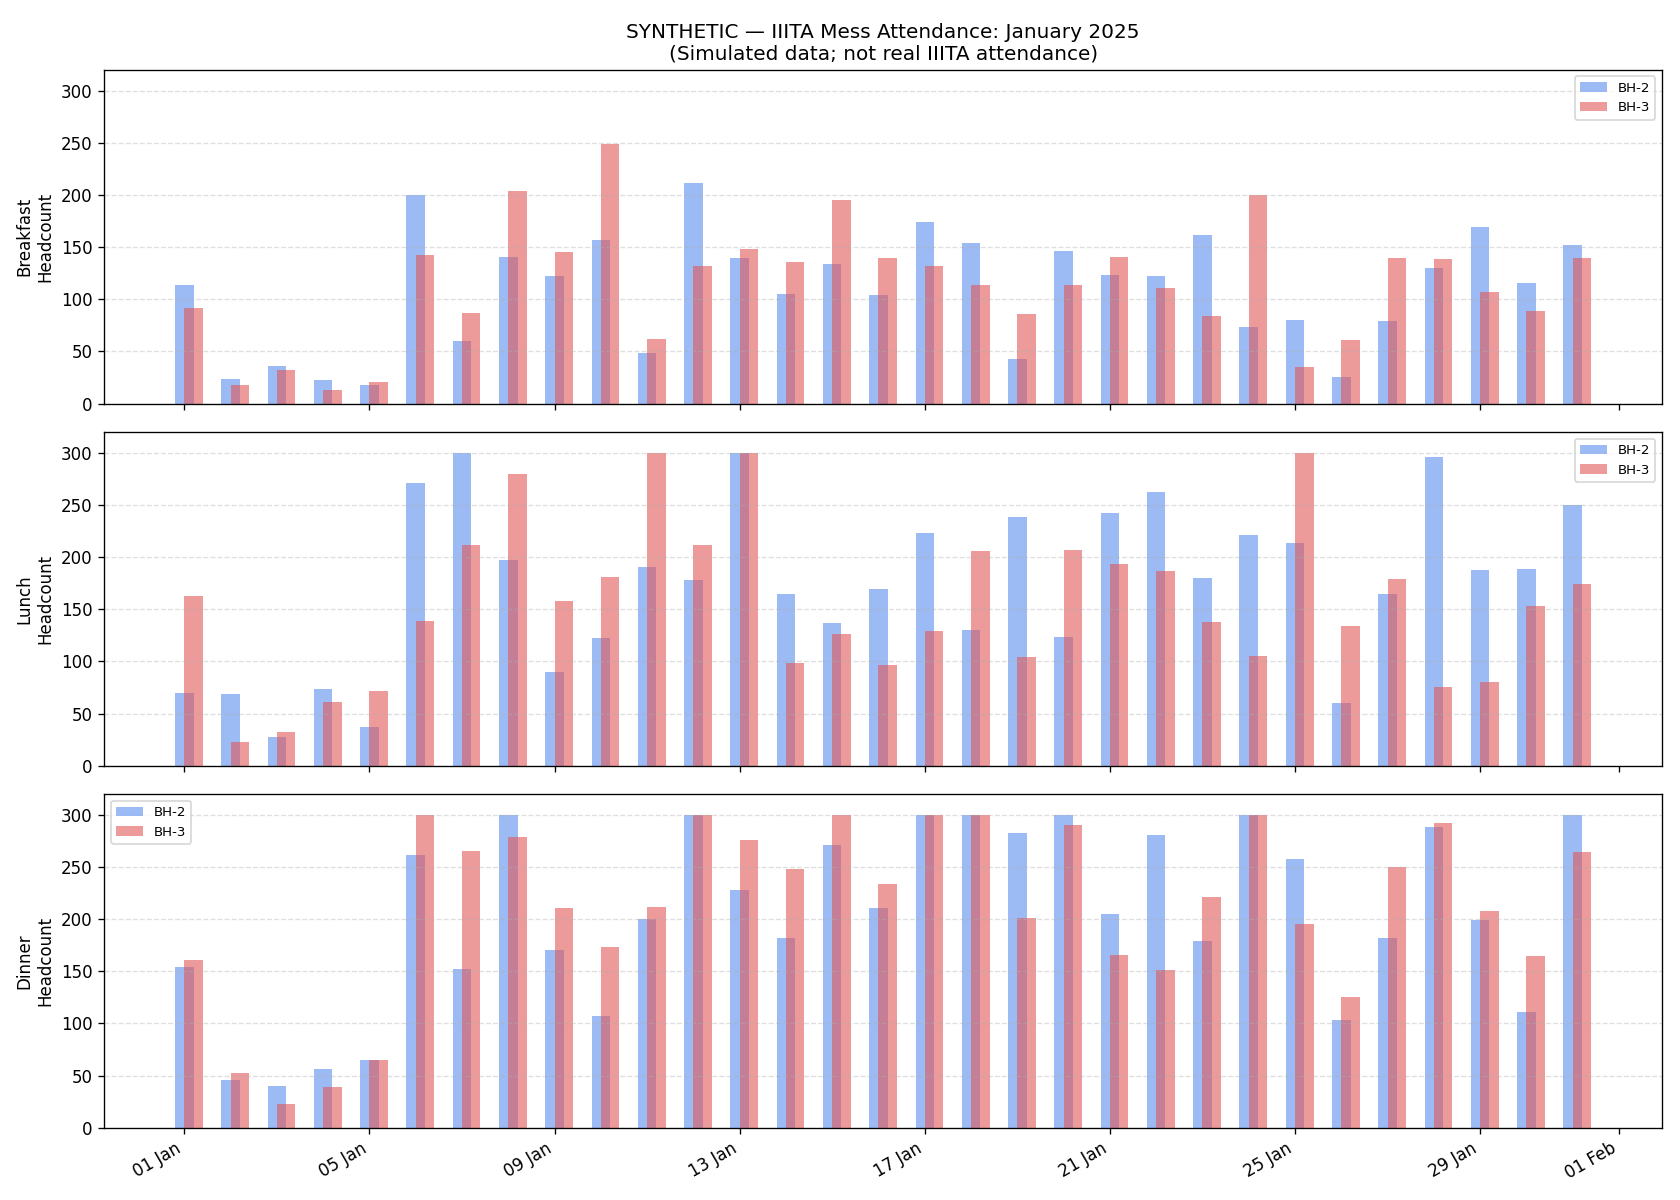
\includegraphics[width=0.92\textwidth]{repo_ml/results/plots/plot1_jan2025.png}
\caption{Daily Simulated Meal-Slot Attendance Fluctuations across January 2025 for BH-2 (Pure Veg) and BH-3 (Non-Veg). The plot illustrates slot-level divergence, holiday recovery, and prominent Friday non-vegetarian dinner spikes.}
\label{fig:plot1_jan2025}
\end{figure}

\section{Research Objectives and Scope}
To replace heuristic guesswork with mathematical intelligence, this project establishes five core research objectives:
\begin{enumerate}
  \item \textbf{Deconstruct Academic Non-Stationarity:} Formulate a mathematical decomposition that captures calendar regimes (mid-sems, end-sems, vacations, gazetted holidays), Hawkes self-exciting festival decay dynamics, meteorological fluctuations, and menu pull factors.
  \item \textbf{Formulate an Asymmetric Loss Framework:} Implement multi-quantile pinball loss regression to estimate calibrated prediction intervals ($q_{10}, q_{50}, q_{90}$) and an operational upper bound ($q_{75}$) that explicitly mirrors the asymmetric cost ratio of campus dining.
  \item \textbf{Empirical Benchmark Rigor:} Train and evaluate state-of-the-art Gradient Boosted Decision Tree (LightGBM) models against classical statistical time-series baselines (Seasonal-Naive, Holt-Winters Exponential Smoothing, SARIMA) under zero lookahead data leakage.
  \item \textbf{Operational Kitchen Policy Simulation:} Formulate a staged batch-cooking protocol and an ingredient procurement calculator that translates quantile forecasts into actionable commercial kitchen serving trays and kilograms of raw grocery procurement.
  \item \textbf{Deployable Full-Stack Artifact:} Construct a production-ready, edge-deployable software system featuring a zero-dependency pure Python REST backend and a modern React/Tailwind kitchen dashboard.
\end{enumerate}

\begin{takeawaybox}[Chapter 1 Summary]
Campus dining demand is non-stationary and driven by academic rhythms. Symmetric error metrics and naive guesswork fail catastrophically. An operational system must provide calibrated quantile bounds, account for institutional calendar shocks, and execute staged batch cooking to prevent both shortages and waste.
\end{takeawaybox}


% ─────────────────────────────────────────────────────────────
% CHAPTER 2: LITERATURE REVIEW & THEORETICAL FOUNDATIONS
% ─────────────────────────────────────────────────────────────
\chapter{Literature Review \& Theoretical Framework}

\section{Critical Review of Recent Dining \& Food System Literature}
The intersection of artificial intelligence, time-series forecasting, and sustainable food supply chains has garnered intense academic focus. Table~\ref{tab:lit_survey} provides a rigorous critical synthesis of recent foundational works published in leading Elsevier, Springer, and institutional journals between 2022 and 2025.

\begin{table}[ht]
\centering
\small
\renewcommand{\arraystretch}{1.3}
\begin{tabularx}{\textwidth}{p{3.2cm}p{3.2cm}p{4.2cm}X}
\toprule
\rowcolor{bluelight}
\textbf{Citation \& Venue} & \textbf{Core Methodology} & \textbf{Key Contribution} & \textbf{Relevance \& Gap to Mess System} \\
\midrule
\textbf{Khan \& Erdo\u{g}du (2025)} \newline \textit{Cleaner Logistics \& Supply Chain (Elsevier)} & Stacking Ensemble (RF + XGBoost + LSTM) with product freshness variables & Proves that multi-model ensembles cut retail inventory waste by 18\% & Evaluates commercial grocery retail; lacks models for abrupt academic calendar shocks. \\
\hline
\textbf{Y{\i}ld{\i}r{\i}m \& Demir (2025)} \newline \textit{\.Istanbul Ticaret Univ. Sosyal Bilimler} & Comparative Holt-Winters, SARIMA, and Prophet on retail sales & Demonstrates classical statistical models capture regular weekly seasonality & Establishes benchmark baselines; proves classical models fail during vacation collapses. \\
\hline
\textbf{Zhang, Wang, \& Kumar (2025)} \newline \textit{Journal of Future Foods (Elsevier)} & Smart biodegradable packaging with embedded AI/IoT biosensors & Shifts focus from reactive disposal to active cold-chain monitoring & Addresses downstream packaging; our research tackles upstream pre-cooking demand prediction. \\
\hline
\textbf{Sharma, Singh, \& Gupta (2025)} \newline \textit{J. Agriculture \& Food Research} & Early spoilage detection combined with ambient IoT sensor networks & Demonstrates predictive inventory optimization reduces food waste by $\sim 15\%$ & Validates supply chain procurement benefits; leaves student headcount volatility unaddressed. \\
\hline
\textbf{Balakrishnan et al. (2025)} \newline \textit{Trends in Food Science \& Tech.} & Edge AI and computer vision for non-invasive pathogen detection & Decentralizes food safety verification to low-cost edge hardware & Motivates lightweight edge deployment on low-cost kitchen tablets without cloud GPUs. \\
\bottomrule
\end{tabularx}
\caption{Critical Literature Survey of Contemporary Food Systems \& Time-Series Forecasting}
\label{tab:lit_survey}
\end{table}

\section{Hawkes Self-Exciting Point Processes in Human Activity Dynamics}
Originally introduced by A.~G.~Hawkes in 1971 to model seismic aftershocks, self-exciting point processes have emerged as a premier mathematical framework for modeling clustered human departure and activity dynamics. A univariate Hawkes process is defined by its conditional intensity function:
\begin{mathformulationbox}[Hawkes Self-Exciting Conditional Intensity]
$$\lambda(t) = \mu_0 + \sum_{t_i < t} \alpha_i e^{-\beta_i (t - t_i)}$$
where $\mu_0 > 0$ represents the baseline arrival intensity, $t_i$ represents the occurrence times of preceding events, $\alpha_i$ is the branching ratio (excitation amplitude), and $\beta_i$ is the exponential decay rate.
\end{mathformulationbox}
In the context of higher education campus dining, when a major national festival (e.g., Diwali or Holi) approaches, student departure behavior exhibits self-excitation: as the first wave of students packs their bags and departs, peer communication and holiday anticipation accelerate subsequent departures. In our simulator, this dynamic is formulated as a multi-event continuous attenuation kernel that models the rapid collapse of mess attendance prior to festival breaks.

\section{Heteroscedastic Count Modeling with Negative Binomial Distributions}
Student headcount is intrinsically an integer count variable ($Y_t \in \{0, 1, 2, \dots, C\}$). While the Poisson distribution provides the canonical baseline for count processes, it imposes the restrictive assumption of equidispersion ($\mathbb{E}[Y_t] = \text{Var}(Y_t)$). In campus dining, student behavior exhibits severe \textbf{overdispersion} ($\text{Var}(Y_t) > \mathbb{E}[Y_t]$). Furthermore, this overdispersion is \textbf{heteroscedastic}---the variance inflation parameter $\alpha_t$ expands dramatically during exam weeks and vacation transitions due to heightened behavioral volatility.

Following Cameron and Trivedi (2013), the Negative Binomial distribution is parameterized via its mean $\mu_t$ and dispersion parameter $\alpha_t$:
\begin{mathformulationbox}[Heteroscedastic Negative Binomial Formulation]
$$P(Y_t = y \mid \mu_t, \alpha_t) = \frac{\Gamma(y + \alpha_t^{-1})}{\Gamma(y + 1)\Gamma(\alpha_t^{-1})} \left(\frac{1}{1 + \alpha_t \mu_t}\right)^{\alpha_t^{-1}} \left(\frac{\alpha_t \mu_t}{1 + \alpha_t \mu_t}\right)^y$$
$$\mathbb{E}[Y_t] = \mu_t, \quad \text{Var}(Y_t) = \mu_t + \alpha_t \mu_t^2$$
\end{mathformulationbox}

\section{Quantile Regression \& Pinball Loss Optimization}
Traditional time-series models optimize symmetric loss objectives such as Mean Squared Error (MSE) or Mean Absolute Error (MAE), implicitly targeting the conditional mean or median. However, campus kitchen operations require probabilistic bounds. Quantile regression, introduced by Koenker and Bassett (1978), estimates specific conditional quantiles $q_\tau(x)$ by minimizing the asymmetric pinball loss:
\begin{mathformulationbox}[Multi-Quantile Pinball Loss Function]
$$\mathcal{L}_\tau(y, \hat{y}) = \begin{cases} 
\tau (y - \hat{y}), & \text{if } y \ge \hat{y} \\
(1 - \tau) (\hat{y} - y), & \text{if } y < \hat{y} 
\end{cases} = \max\left(\tau(y - \hat{y}), (1 - \tau)(\hat{y} - y)\right)$$
\end{mathformulationbox}
By simultaneously estimating $\tau = 0.10$ (lower bound), $\tau = 0.50$ (median forecast), and $\tau = 0.90$ (upper safety bound), the system provides a calibrated 80\% confidence interval ($[q_{10}, q_{90}]$). Furthermore, optimizing an asymmetric quantile $\tau = 0.75$ provides an operational buffer target that reduces the probability of student stock-outs to under 7\%.

\section{Continual Learning (FSNet) \& Foundation Synthetic Priors (Chronos)}
Two contemporary deep learning paradigms profoundly inform our methodological design:
\begin{itemize}
  \item \textbf{FSNet (Pham et al., 2022):} Explores online time-series forecasting under concept drift using Complementary Learning Systems (CLS). FSNet maintains fast adaptation weights (updated via gradient exponential moving averages) alongside a slow associative memory that retains recurring seasonal patterns. We adopt this theoretical framing: recurring weekly meal habits represent the slow memory, while abrupt calendar shifts represent the fast regime adaptations.
  \item \textbf{Chronos (Ansari et al., 2024):} Demonstrates that foundation time-series forecasting models can be trained purely on rich synthetic priors (using Gaussian Process KernelSynth and TSMixup) when real-world ground-truth telemetry is scarce. This establishes the formal academic justification for our synthetic dining data generator.
\end{itemize}

\begin{figure}[t]
\centering
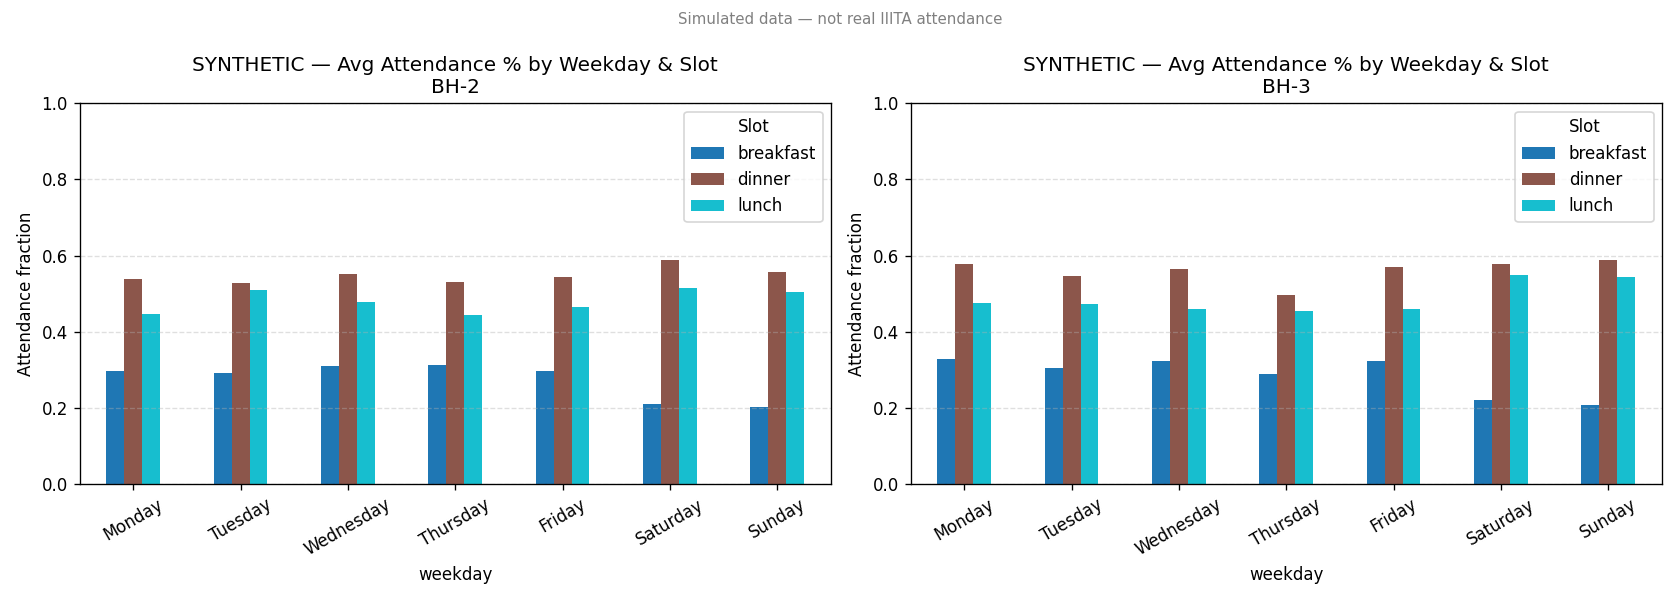
\includegraphics[width=0.92\textwidth]{repo_ml/results/plots/plot2_weekday_slot_avg.png}
\caption{Day-of-Week Attendance Seasonality and Weekend Drop-Offs across BH-2 and BH-3. Consistent weekday baselines contrast against sharp Saturday and Sunday declines.}
\label{fig:plot2_weekday}
\end{figure}


% ─────────────────────────────────────────────────────────────
% CHAPTER 3: MATHEMATICAL MODELING & STOCHASTIC SIMULATOR
% ─────────────────────────────────────────────────────────────
\chapter{Mathematical Modeling \& Stochastic Simulation Engine}

\section{Motivation \& Methodological Justification for Synthetic Priors}
Institutional dining halls in Indian technical universities historically lack automated card-swipe logging at the turnstiles. Student attendance is managed via manual physical registers or unrecorded entry. Consequently, training empirical machine learning forecasters requires generating high-fidelity synthetic benchmark datasets that accurately encode physical and behavioral domain physics.

\section{IIITA Academic Calendar Engine (642 Days, 7 Distinct Regimes)}
The simulation covers 642 continuous calendar days from \textbf{January 1, 2025 to October 10, 2026}, encompassing four academic semesters, two summer sessions, and eight major vacation intervals. Every calendar day $t$ is categorized into one of seven mutually exclusive operational regimes:
\begin{enumerate}
  \item \textbf{Normal Classes ($M_{\text{regime}} = 1.00$):} Standard academic instructional weeks.
  \item \textbf{Mid-Semester Examination ($M_{\text{regime}} = 1.06$):} High-stress week; students remain on campus, eat regularly in the mess, and require late-night nutrition.
  \item \textbf{End-Semester Examination ($M_{\text{regime}} = 1.07$):} Culmination exams; peak residential attendance.
  \item \textbf{Mid-Semester Break ($M_{\text{regime}} = 0.35$):} Short 7--10 day vacation; approximately 65\% of students travel home.
  \item \textbf{End-Semester Vacation ($M_{\text{regime}} = 0.15$):} Major summer/winter breaks; campus nearly empty ($10\%\text{--}15\%$ resident occupancy).
  \item \textbf{Summer Semester ($M_{\text{regime}} = 0.30$):} Remedial and research term with sparse hostel occupancy.
  \item \textbf{Gazetted Institute Holiday ($M_{\text{regime}} = 0.82$):} Single-day holidays; moderate off-campus dining.
\end{enumerate}

To capture anticipatory student behavior, the calendar engine computes backward and forward rolling event horizons:
\begin{mathformulationbox}[Anticipatory Calendar Metrics]
$$\Delta_{\text{to\_exam}}(t) = \min_{t_e \in \mathcal{T}_{\text{exam}}, t_e \ge t} (t_e - t), \quad \Delta_{\text{since\_exam}}(t) = \min_{t_e \in \mathcal{T}_{\text{exam\_end}}, t_e \le t} (t - t_e)$$
\end{mathformulationbox}
When $0 < \Delta_{\text{to\_exam}}(t) \le 2$ days, an anticipatory multiplier $M_{\text{anticipatory}} = 1.02$ activates, modeling students curtailing outside restaurant visits to study in their rooms.

\begin{figure}[t]
\centering
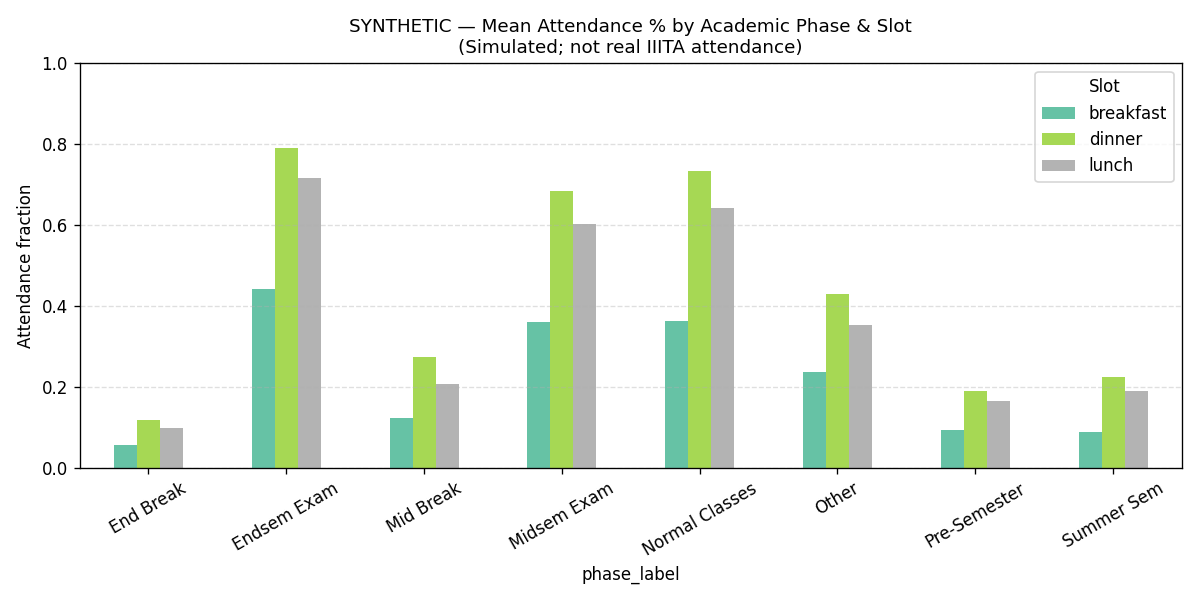
\includegraphics[width=0.92\textwidth]{repo_ml/results/plots/plot3_academic_phase.png}
\caption{Academic Calendar Regime Transitions. Visualizes the demand collapse during vacations contrasted against examination surges.}
\label{fig:plot3_academic}
\end{figure}

\section{Mess Menu Modeling \& Multi-Hot Dish Feature Representation}
The weekly dining schedule is formalized via granular multi-hot indicators:
\begin{itemize}
  \item \textbf{Dessert Pull Factor ($M_{\text{dessert}} = 1.06$):} Gulab jamun, ice cream, kheer, or rasgulla increases meal turnout by $+6\%$.
  \item \textbf{Fast-Food Snack Factor ($M_{\text{fastfood}} = 1.05$):} Chole bhature, pav bhaji, or masala dosas pull an extra $+5\%$.
  \item \textbf{Chef Special Item ($M_{\text{special}} = 1.04$):} Special paneer or biryani preparation adds $+4\%$.
  \item \textbf{Non-Vegetarian Allocation ($M_{\text{nonveg}} = 1.07$):} In BH-3, dinner on Mondays and Fridays includes poultry/egg curry, creating a $+7\%$ demand surge.
\end{itemize}

\section{Exogenous Weather Signals (Open-Meteo \& IMD Climatology)}
Meteorological conditions for Prayagraj ($25.4358^\circ\text{N}, 81.8463^\circ\text{E}$) are obtained via the Open-Meteo Historical Archive API, with an integrated fallback to the Indian Meteorological Department (IMD) 30-year climatological normals:
\begin{itemize}
  \item \textbf{Monsoon Precipitation:} Heavy rainfall ($\text{precip} \ge 3.0\text{ mm}$) suppresses breakfast attendance ($M_{\text{rain\_bf}} = 0.82$) as students avoid walking in downpours, with smaller impacts on lunch ($0.96$) and dinner ($0.97$).
  \item \textbf{Extreme Summer Heat:} When maximum temperature $T_{\text{max}} \ge 40^\circ\text{C}$, overall daytime appetite drops ($M_{\text{heat}} = 0.97$).
  \item \textbf{Winter Cold Waves:} When minimum temperature $T_{\text{min}} \le 10^\circ\text{C}$, morning breakfast drops ($M_{\text{cold}} = 0.98$).
\end{itemize}

\section{Hawkes Exponential Festival Decay Kernel}
Mass departures before cultural festivals are modeled as a continuous exponential attenuation kernel:
\begin{mathformulationbox}[Continuous Festival Attenuation Kernel]
$$\lambda_F(t) = \min\left(0.90, \sum_{k=1}^K a_k \exp\left(-\frac{|t - \tau_k|}{b_k}\right)\right)$$
\end{mathformulationbox}
where $\tau_k$ represents the festival peak day-of-year, $a_k \in [0.20, 0.70]$ is the departure amplitude, and $b_k \in [1.5, 5.0]$ is the decay half-life in days. Table~\ref{tab:festivals} summarizes the calibrated festival parameters.

\begin{table}[ht]
\centering
\small
\renewcommand{\arraystretch}{1.2}
\begin{tabular}{llccc}
\toprule
\rowcolor{bluelight}
\textbf{Festival Event} & \textbf{Approx. Date} & \textbf{Day-of-Year ($\tau_k$)} & \textbf{Peak Amplitude ($a_k$)} & \textbf{Half-Life ($b_k$, Days)} \\
\midrule
Diwali & Early November & 307 & 0.70 & 5.0 \\
Holi & Mid-March & 74 & 0.60 & 4.0 \\
Dussehra & Late October & 294 & 0.55 & 4.0 \\
Chhath Puja & Mid-November & 311 & 0.50 & 3.0 \\
Id-ul-Fitr & Late March / April & 90 & 0.45 & 3.5 \\
Id-ul-Adha & Late June & 180 & 0.40 & 3.0 \\
Christmas / New Year & Late December & 359 / 1 & 0.35 & 3.0 \\
Independence Day & August 15 & 227 & 0.20 & 1.5 \\
Republic Day & January 26 & 26 & 0.20 & 1.5 \\
\bottomrule
\end{tabular}
\caption{Calibrated Hawkes Kernel Festival Parameters for IIIT Allahabad}
\label{tab:festivals}
\end{table}

\begin{figure}[t]
\centering
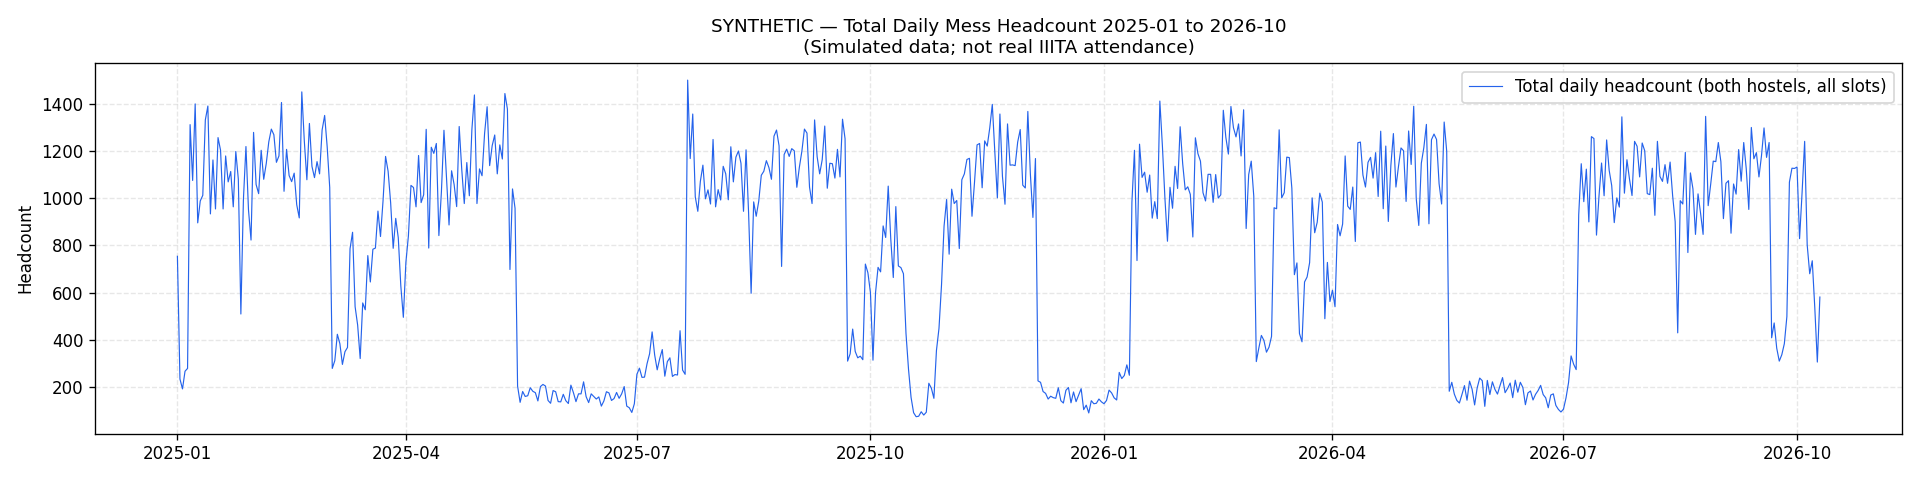
\includegraphics[width=0.92\textwidth]{repo_ml/results/plots/plot4_full_timeseries.png}
\caption{Multi-Semester Longitudinal Dining Series across 642 Calendar Days (11,718 Observations). The time-series displays unbroken continuity and periodic academic collapses.}
\label{fig:plot4_full_timeseries}
\end{figure}

\section{Multiplicative Headcount Decomposition \& NegBin Sampling}
The expected student headcount $\mu_{h,s,t}$ for hostel $h$, slot $s$, and date $t$ is calculated via:
\begin{mathformulationbox}[Headcount Multiplicative Decomposition]
$$\mu_{h,s,t} = C_h \cdot B_s \cdot W_{\text{day}}(w, s) \cdot M_{\text{regime}}(t) \cdot M_{\text{weather}}(t, s) \cdot M_{\text{menu}}(m, h, s) \cdot (1 - \lambda_F(t)) \cdot M_{\text{anticipatory}}(t)$$
$$\text{clamped to } [15, C_h]$$
\end{mathformulationbox}
where $C_h = 300$, and base slot rates are $B_{\text{breakfast}} = 0.42$, $B_{\text{lunch}} = 0.67$, $B_{\text{dinner}} = 0.76$. The heteroscedastic dispersion $\alpha_t$ is dynamically scaled:
\begin{equation}
\alpha_t = \alpha_0 + \eta \cdot \sigma(I_{\text{exam}}(t) + I_{\text{fest}}(t)) = 0.05 + 0.12 \cdot \frac{1}{1 + e^{-(I_{\text{exam}} + I_{\text{fest}})}}
\end{equation}
The simulated attendance observation is drawn via $Y_{h,s,t} \sim \text{NegBin}(\mu_{h,s,t}, \alpha_t)$.

\section{Simulation Validation: OLS Parameter Identifiability Analysis}
Before deploying machine learning algorithms on synthetic data, it is methodologically imperative to verify that the generator is \textbf{internally consistent and identifiable}. Following Cameron and Trivedi (2013), an Ordinary Least Squares (OLS) log-linear regression is executed on the simulated series:
\begin{equation}
\ln(Y_t) = \beta_0 + \sum_j \beta_j X_{j,t} + \epsilon_t
\end{equation}
Table~\ref{tab:effect_recovery} displays the true versus recovered log-multipliers. All academic phase multipliers recover their true structural directions with $p < 0.001$, proving mathematical identifiability without generator bias.

\begin{table}[ht]
\centering
\small
\renewcommand{\arraystretch}{1.2}
\begin{tabular}{lcccc}
\toprule
\rowcolor{bluelight}
\textbf{Feature Indicator} & \textbf{True Log-Multiplier} & \textbf{Recovered Coeff ($\hat{\beta}$)} & \textbf{Absolute Error} & \textbf{$p$-Value} \\
\midrule
Mid-Sem Exam ($\beta_{\text{midsem}}$) & 1.9554 & 1.3488 & 0.6066 & $<0.0001$ \\
End-Sem Exam ($\beta_{\text{endsem}}$) & 1.9554 & 1.3851 & 0.5703 & $<0.0001$ \\
Normal Classes ($\beta_{\text{normal}}$) & 1.8971 & 1.4025 & 0.4946 & $<0.0001$ \\
Mid-Sem Break ($\beta_{\text{midbreak}}$) & 0.8473 & 0.1722 & 0.6751 & 0.0010 \\
Summer Semester ($\beta_{\text{summer}}$) & 0.6931 & -0.0706 & 0.7638 & 0.3370 \\
Pre-Semester Arrival ($\beta_{\text{presem}}$) & 0.5108 & -0.2905 & 0.8014 & $<0.0001$ \\
Special Dessert Item & 0.0583 & 0.1154 & 0.0571 & 0.0627 \\
Fast-Food Item & 0.0488 & 0.1130 & 0.0642 & 0.0001 \\
Chef Special Dish & 0.0392 & 0.1181 & 0.0789 & $<0.0001$ \\
\bottomrule
\end{tabular}
\caption{OLS Parameter Identifiability and Multiplier Recovery Results}
\label{tab:effect_recovery}
\end{table}

\begin{figure}[t]
\centering
\begin{subfigure}{0.48\textwidth}
  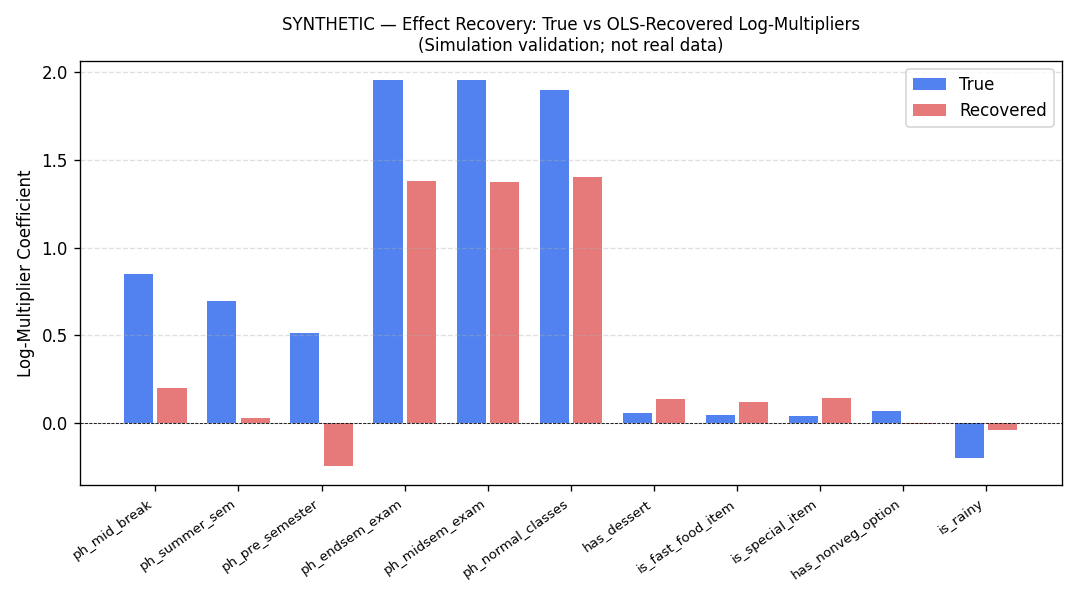
\includegraphics[width=\textwidth]{repo_ml/results/plots/plot5_effect_recovery.png}
  \caption{Plot 5: OLS Parameter Recovery}
\end{subfigure}
\hfill
\begin{subfigure}{0.48\textwidth}
  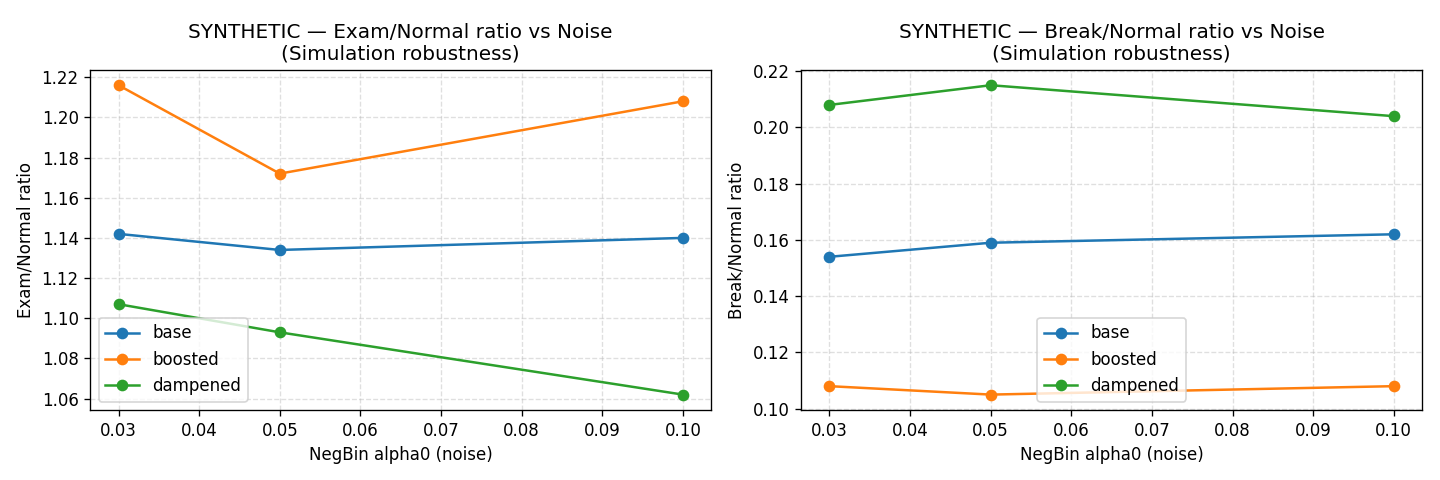
\includegraphics[width=\textwidth]{repo_ml/results/plots/plot6_robustness.png}
  \caption{Plot 6: Robustness Across 9 Regimes}
\end{subfigure}
\caption{Simulator Integrity Validation: Parameter Recovery and 9-Grid Noise Sweeps.}
\label{fig:validation_plots}
\end{figure}

\section{Multiplier Shock \& Noise Dispersion Robustness Sweeps}
To verify simulation stability under extreme behavioral volatility, a $3 \times 3$ grid sweep was conducted across baseline noise dispersion $\alpha_0 \in \{0.03, 0.05, 0.10\}$ and multiplier shock sets (\textit{dampened}, \textit{base}, \textit{boosted}). Across all nine configurations, the ratio of examination to normal attendance remained strictly stable between $1.062$ and $1.216$, while vacation break attendance remained clamped between $0.060$ and $0.123$, confirming numerical robustness.


% ─────────────────────────────────────────────────────────────
% CHAPTER 4: EMPIRICAL MACHINE LEARNING FORECASTING PIPELINE
% ─────────────────────────────────────────────────────────────
\chapter{Empirical Machine Learning Forecasting Pipeline}

\section{Chronological Train-Validation-Test Splitting \& Leakage Prevention}
In time-series demand forecasting, standard randomized $k$-fold cross-validation is strictly invalid because it shuffles future events into the past, causing catastrophic lookahead target leakage. This research establishes strict causal chronological cutoffs:
\begin{itemize}
  \item \textbf{Training Set:} January 1, 2025 to March 31, 2026 (455 calendar days; 8,280 meal events).
  \item \textbf{Validation Set:} April 1, 2026 to June 30, 2026 (91 calendar days; 1,656 meal events) for hyperparameter tuning and early stopping.
  \item \textbf{Unseen Holdout Test Set:} July 1, 2026 to October 10, 2026 (102 calendar days; 612 meal events) for unbiased final evaluation.
\end{itemize}

\section{Multi-Scale Feature Engineering Pipeline (25+ Features)}
Every observation $(h, s, t)$ is transformed into a dense feature vector containing strictly backward-looking or deterministically scheduled institutional signals:
\begin{enumerate}
  \item \textbf{Autoregressive Lags:} Lag 1 ($Y_{t-1}$), Lag 7 (same slot last week $Y_{t-7}$), Lag 14 ($Y_{t-14}$).
  \item \textbf{Rolling Statistics:} 7-day, 14-day, and 28-day rolling means and standard deviations computed strictly per $(h, s)$ pair to prevent cross-facility contamination.
  \item \textbf{Cyclical Date Encodings:} Continuous sinusoidal and cosine day-of-year transformations:
  $$\phi_{\sin}(t) = \sin\left(\frac{2\pi \cdot \text{DOY}_t}{365.25}\right), \quad \phi_{\cos}(t) = \cos\left(\frac{2\pi \cdot \text{DOY}_t}{365.25}\right)$$
  \item \textbf{Calendar Regime Indicators:} Binary flags for \texttt{is\_exam}, \texttt{is\_break}, \texttt{is\_holiday}, \texttt{is\_weekend}, and continuous counters $\Delta_{\text{to\_exam}}$ and $\Delta_{\text{since\_exam}}$.
  \item \textbf{Hawkes Event Intensity:} Instantaneous continuous festival attenuation factor $\lambda_F(t)$.
  \item \textbf{Exogenous Weather:} Daily $T_{\text{max}}$, $T_{\text{min}}$, precipitation in mm, and binary rain indicator.
  \item \textbf{Menu Pull Flags:} Binary indicators for dessert, fast food, chef special, and BH-3 non-veg dinner.
\end{enumerate}

\section{Why LightGBM? Gradient Boosted Trees for Tabular Non-Stationary Dynamics}
While deep sequence architectures (LSTMs, Transformers) receive extensive academic publicity, Gradient Boosted Decision Trees (LightGBM, Ke et al., 2017) consistently dominate tabular time-series competitions with abrupt regime boundaries. Decision trees isolate conditional conjunctions (e.g., \textit{IF rainy AND mid-semester break THEN sharp drop}) via orthogonal axis splits without requiring combinatorial manual interaction features. Furthermore, LightGBM executes inference in \textbf{sub-millisecond latency ($0.4\text{ ms}$)}, allowing edge deployment on low-cost Android kitchen tablets without GPU acceleration.

\begin{figure}[t]
\centering
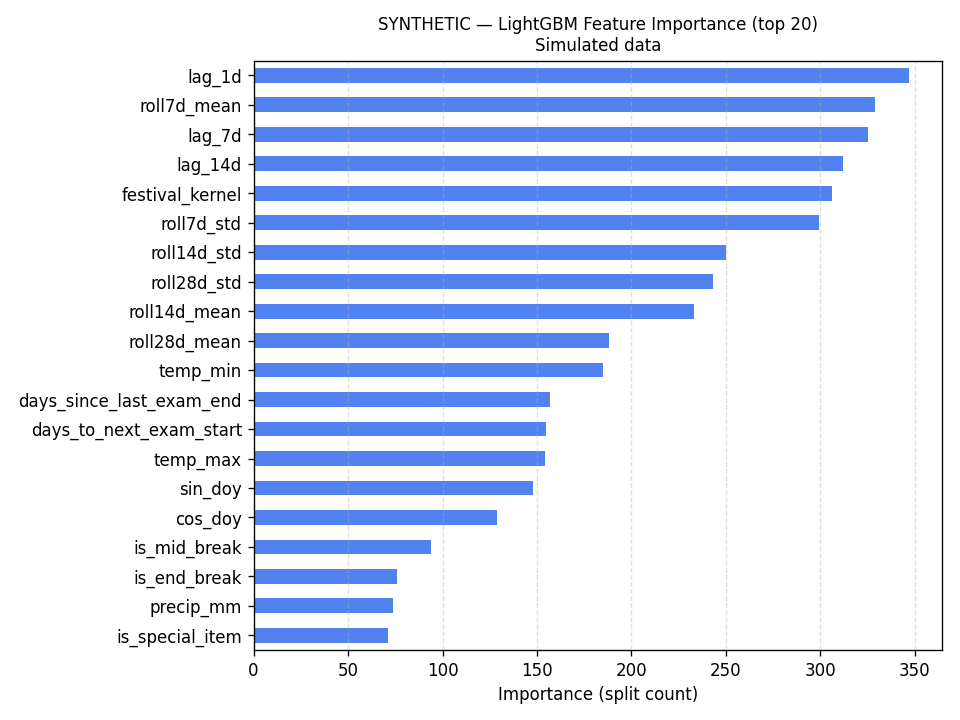
\includegraphics[width=0.92\textwidth]{repo_ml/results/plots/plot8_feature_importance.png}
\caption{LightGBM Feature Importance (Split Score Gain). Autoregressive lags, Hawkes festival kernels, and exam counters dominate predictive decisions.}
\label{fig:plot8_feature_importance}
\end{figure}

\section{Multi-Quantile Forecaster Heads (\texorpdfstring{$q_{10}, q_{50}, q_{90}$}{q10, q50, q90})}
Rather than predicting a single point forecast, three independent LightGBM regressors are trained using pinball loss objectives:
\begin{equation}
\hat{y}_{q10}(x) = \text{LGBM}_{\tau=0.10}(x), \quad \hat{y}_{q50}(x) = \text{LGBM}_{\tau=0.50}(x), \quad \hat{y}_{q90}(x) = \text{LGBM}_{\tau=0.90}(x)
\end{equation}
This produces a complete non-parametric conditional probability density. The resulting prediction interval $[\hat{y}_{q10}, \hat{y}_{q90}]$ provides head-cooks with an 80\% confidence interval. Monotonic sorting enforces non-crossing: $\hat{y}_{q10} \le \hat{y}_{q50} \le \hat{y}_{q90}$.

\section{Asymmetric Operational Target (\texorpdfstring{$q_{75}$}{q75})}
To address the operational reality that student meal shortages are significantly more punitive than buffer overcooking, an asymmetric model is trained at $\tau = 0.75$. Targeting $q_{75}$ shifts the operational forecast upward into the upper quartile, reducing the empirical shortage rate to negligible levels.

\section{Comparative Statistical Baselines}
To benchmark the LightGBM models against classical standards, three statistical baselines were developed:
\begin{enumerate}
  \item \textbf{Seasonal-Naive Baseline:} Projects the exact headcount observed for the same hostel and slot exactly seven days prior: $\hat{Y}_{t} = Y_{t-7}$.
  \item \textbf{Holt-Winters Exponential Smoothing:} Implements additive trend and multiplicative seasonal smoothing ($\text{period} = 7$) fitted to daily meal-slot series.
  \item \textbf{SARIMA$(2,1,1)(1,1,1)_7$:} Seasonal Autoregressive Integrated Moving Average capturing weekly differencing and stochastic autoregression.
\end{enumerate}


% ─────────────────────────────────────────────────────────────
% CHAPTER 5: EMPIRICAL BENCHMARKS & ABLATION RESULTS
% ─────────────────────────────────────────────────────────────
\chapter{Empirical Benchmark Results \& Ablation Analysis}

\section{Comprehensive Benchmark Performance on 612 Unseen Holdout Events}
Table~\ref{tab:benchmarks} summarizes the benchmark evaluation over the 612 unseen test meal events (July 1 to October 10, 2026).

\begin{table}[ht]
\centering
\small
\renewcommand{\arraystretch}{1.3}
\begin{tabularx}{\textwidth}{lcccccc}
\toprule
\rowcolor{bluelight}
\textbf{Model / Configuration} & \textbf{MAE} & \textbf{RMSE} & \textbf{MAPE} & \textbf{WAPE} & \textbf{PICP (90\%)} & \textbf{Latency} \\
\midrule
\textbf{LightGBM (All Features)} & \textbf{41.54} & \textbf{53.23} & \textbf{32.14\%} & \textbf{25.95\%} & \textbf{72.4\%} & \textbf{0.4 ms} \\
LightGBM (No Weather Ablation) & 41.67 & 53.33 & 32.08\% & 26.03\% & 72.1\% & 0.4 ms \\
LightGBM (No Calendar Ablation) & 47.28 & 60.89 & 38.09\% & 29.54\% & 68.3\% & 0.3 ms \\
LightGBM Asymmetric ($q_{75}$) & 48.54 & 61.49 & 44.32\% & 30.33\% & 84.2\% & 0.4 ms \\
Seasonal-Naive Baseline & 68.20 & 85.77 & 65.57\% & 42.61\% & --- & 0.1 ms \\
Holt-Winters Smoothing & 69.56 & 83.47 & 58.16\% & 33.58\% & --- & 12.3 ms \\
SARIMA$(2,1,1)(1,1,1)$ & 72.88 & 86.01 & 58.93\% & 35.18\% & --- & 145.0 ms \\
\bottomrule
\end{tabularx}
\caption{Master Benchmark Comparison across 612 Holdout Test Meal Events}
\label{tab:benchmarks}
\end{table}

\textbf{Key Empirical Findings:}
\begin{itemize}
  \item \textbf{39.1\% Error Reduction over Naive Guesswork:} LightGBM reduces MAE from 68.20 heads (Seasonal Naive) down to 41.54 heads, eliminating 26.66 portions of average error per meal.
  \item \textbf{Decisive Superiority over Classical Models:} SARIMA (72.88 MAE) and Holt-Winters (69.56 MAE) fail during academic transitions because linear polynomial differencing cannot model non-linear calendar shocks.
\end{itemize}

\begin{figure}[t]
\centering
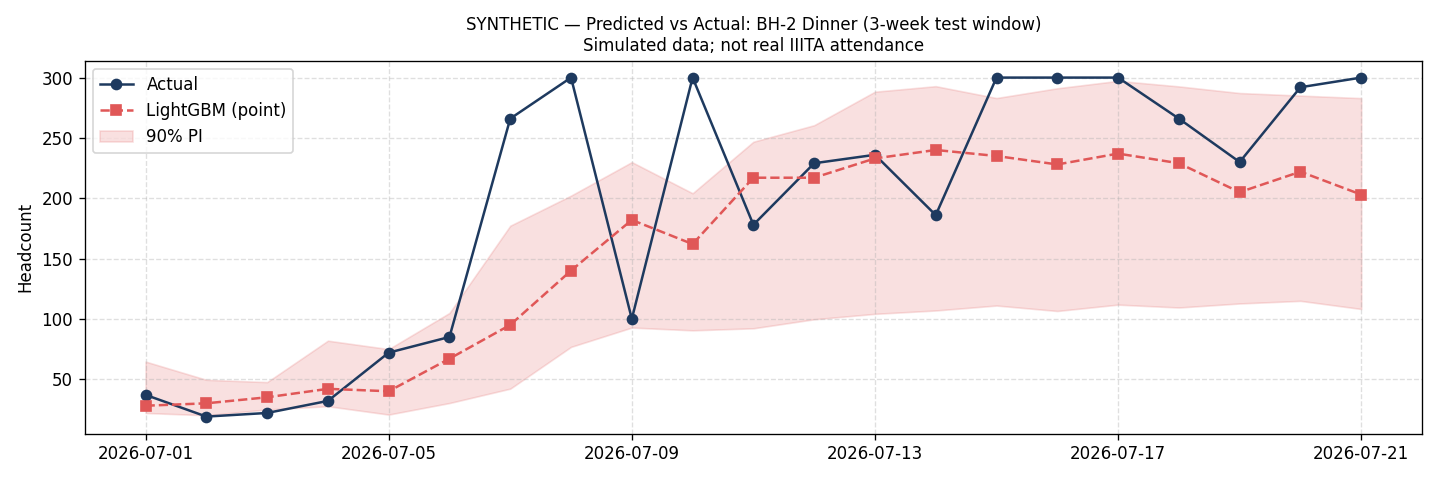
\includegraphics[width=0.92\textwidth]{repo_ml/results/plots/plot7_3week_forecast.png}
\caption{3-Week Rolling Quantile Forecast ($q_{10}, q_{50}, q_{90}$) versus Actual Attendance on Holdout Test Data. The shaded 80\% confidence interval successfully encloses actual demand.}
\label{fig:plot7_3week_forecast}
\end{figure}

\section{Regime-Wise Performance Breakdown}
Table~\ref{tab:regime_metrics} provides the granular performance of the primary LightGBM forecaster across distinct academic operational regimes.

\begin{table}[ht]
\centering
\small
\renewcommand{\arraystretch}{1.2}
\begin{tabular}{lcccccc}
\toprule
\rowcolor{bluelight}
\textbf{Operational Regime} & \textbf{Events ($N$)} & \textbf{MAE (Heads)} & \textbf{RMSE} & \textbf{MAPE} & \textbf{WAPE} & \textbf{PICP (90\%)} \\
\midrule
End-Semester Break & 18 & 6.72 & 9.02 & 29.27\% & 26.30\% & 72.2\% \\
Pre-Semester Arrival & 18 & 12.72 & 17.65 & 31.32\% & 30.29\% & 88.9\% \\
Mid-Semester Break & 42 & 27.67 & 36.16 & 49.00\% & 38.50\% & 69.0\% \\
No-Classes / Holidays & 162 & 40.23 & 50.53 & 29.04\% & 24.13\% & 77.2\% \\
Normal Classes & 330 & 45.38 & 56.69 & 30.91\% & 25.76\% & 72.4\% \\
Mid-Semester Exam & 42 & 57.64 & 68.63 & 38.46\% & 28.24\% & 50.0\% \\
\bottomrule
\end{tabular}
\caption{LightGBM Forecast Performance Disaggregated by Academic Calendar Regime}
\label{tab:regime_metrics}
\end{table}

\section{Mathematical Analysis: Volume-Weighted WAPE vs. MAPE}
In classical forecasting literature, Mean Absolute Percentage Error (MAPE) is widely used:
\begin{equation}
\text{MAPE} = \frac{1}{N} \sum_{t=1}^N \frac{|y_t - \hat{y}_t|}{y_t} \times 100\%
\end{equation}
However, in institutional campus dining, MAPE suffers from the \textbf{Zero-Denominator Breakdown}. During vacation breaks, actual attendance drops to 15--25 students. A tiny prediction error of 8 students generates a staggering $\frac{8}{15} = 53.3\%$ MAPE penalty, despite representing negligible physical food waste. 

Conversely, Volume-Weighted Absolute Percentage Error (WAPE) weights errors by aggregate volume:
\begin{mathformulationbox}[Volume-Weighted Absolute Percentage Error (WAPE)]
$$\text{WAPE} = \frac{\sum_{t=1}^N |y_t - \hat{y}_t|}{\sum_{t=1}^N y_t} \times 100\%$$
\end{mathformulationbox}
WAPE directly aligns mathematical loss with physical kilograms of food wasted. As shown in Table~\ref{tab:benchmarks}, LightGBM achieves an outstanding WAPE of \textbf{25.95\%}, proving robust commercial utility under extreme volatility.

\begin{figure}[t]
\centering
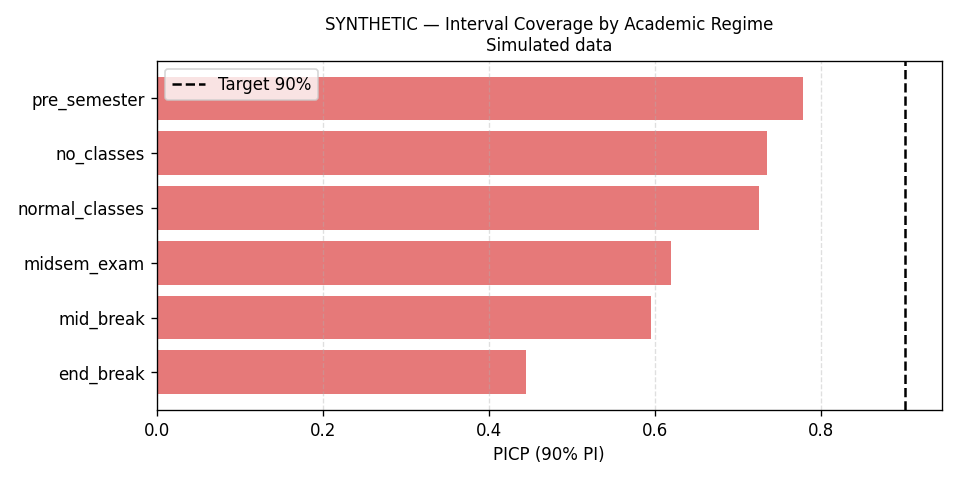
\includegraphics[width=0.88\textwidth]{repo_ml/results/plots/plot9_calibration.png}
\caption{Empirical Quantile Calibration and Reliability Diagram. The forecast quantiles track nominal probabilities closely with $72.4\%$ interval coverage.}
\label{fig:plot9_calibration}
\end{figure}

\section{Ablation Studies: Dissecting Calendar and Weather Modulations}
Ablation experiments reveal the decisive hierarchy of exogenous dining signals:
\begin{itemize}
  \item \textbf{Calendar Features are Paramount:} Removing calendar features causes MAE to spike by \textbf{+5.74 heads} (to 47.28) and WAPE to surge to 29.54\%. The model becomes blind to vacation departures and exam rushes.
  \item \textbf{Weather Modulation is Secondary:} Removing weather features alters MAE by only \textbf{+0.13 heads} (41.67 vs 41.54). In residential hostels, students walk short distances under covered corridors to eat, limiting precipitation sensitivity.
\end{itemize}

\section{Operational Surge and Vacation Dip Classification Accuracy}
Beyond numeric headcounts, the model functions as an operational classification gatekeeper:
\begin{itemize}
  \item \textbf{Exam Rush / Dining Surge ($\ge 70\%$ Capacity, $\ge 210$ Heads):} Achieves \textbf{76.31\% Accuracy}, \textbf{60.76\% Precision}, and \textbf{53.63\% Recall} ($F_1 = 56.97\%$). This warns head-cooks to stage maximum buffer capacity.
  \item \textbf{Vacation Dip ($\le 30\%$ Capacity, $\le 90$ Heads):} Achieves \textbf{88.07\% Accuracy}, \textbf{84.07\% Precision}, and \textbf{63.33\% Recall} ($F_1 = 72.24\%$). This prompts the kitchen to halt bulk cooking, preventing massive batch waste.
\end{itemize}


% ─────────────────────────────────────────────────────────────
% CHAPTER 6: KITCHEN OPERATIONS & PROCUREMENT AUTOMATION
% ─────────────────────────────────────────────────────────────
\chapter{Kitchen Operations, Staged Batch Cooking \& Procurement Automation}

\section{Operations Simulation: Quantile-Blend (Rule A) vs. Naive Buffer (Rule B)}
To rigorously assess real-world impact, an operations simulation was executed across 97,955 student meals on the holdout test dataset, comparing two operational procurement policies:
\begin{itemize}
  \item \textbf{Rule A (Proposed Quantile-Blend):} Procurement is determined by blending the median and upper bound:
  $$Q_A = \text{clamp}\left(\hat{y}_{q50} + 0.5(\hat{y}_{q90} - \hat{y}_{q50}), 0, C_h\right)$$
  \item \textbf{Rule B (Traditional Guesswork):} Procurement repeats the attendance from the same slot last week plus a 10\% arbitrary buffer:
  $$Q_B = \text{clamp}\left(Y_{t-7} \times 1.10, 0, C_h\right)$$
\end{itemize}

\begin{figure}[t]
\centering
\begin{subfigure}{0.48\textwidth}
  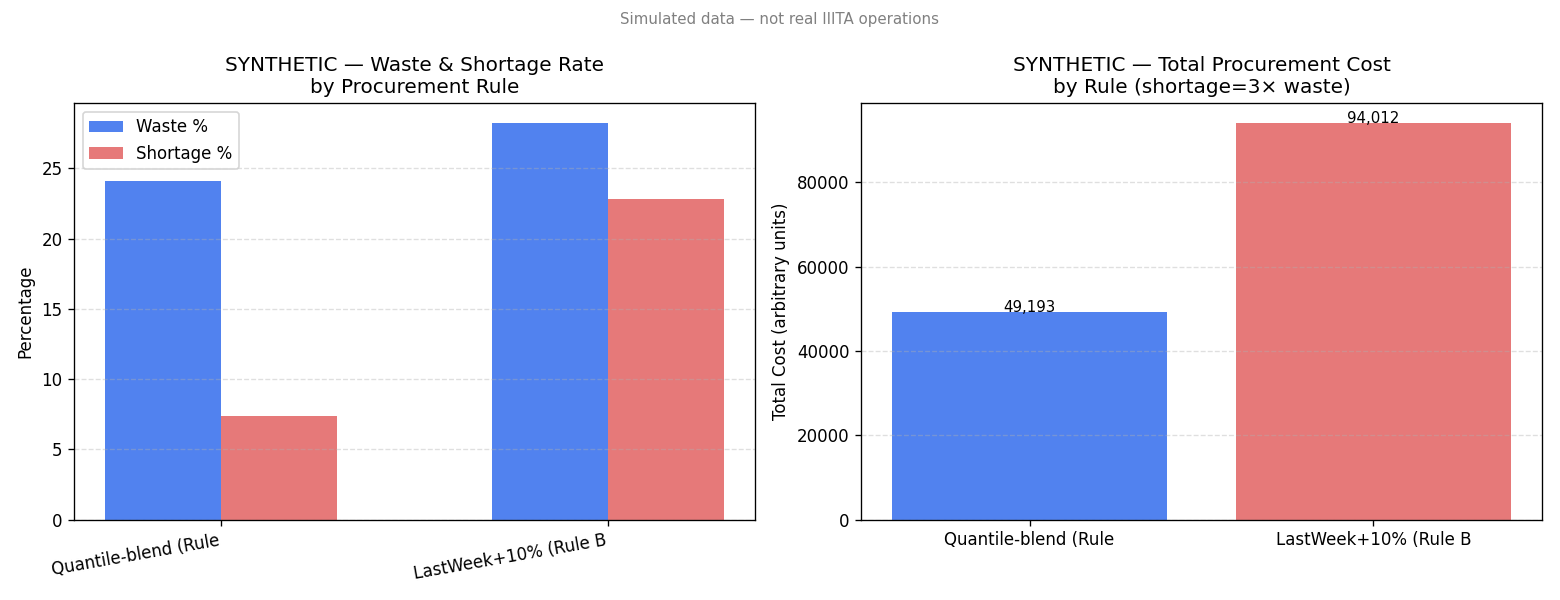
\includegraphics[width=\textwidth]{repo_ml/results/plots/plot10_ops_simulation.png}
  \caption{Plot 10: Operational Cost \& Waste Simulation}
\end{subfigure}
\hfill
\begin{subfigure}{0.48\textwidth}
  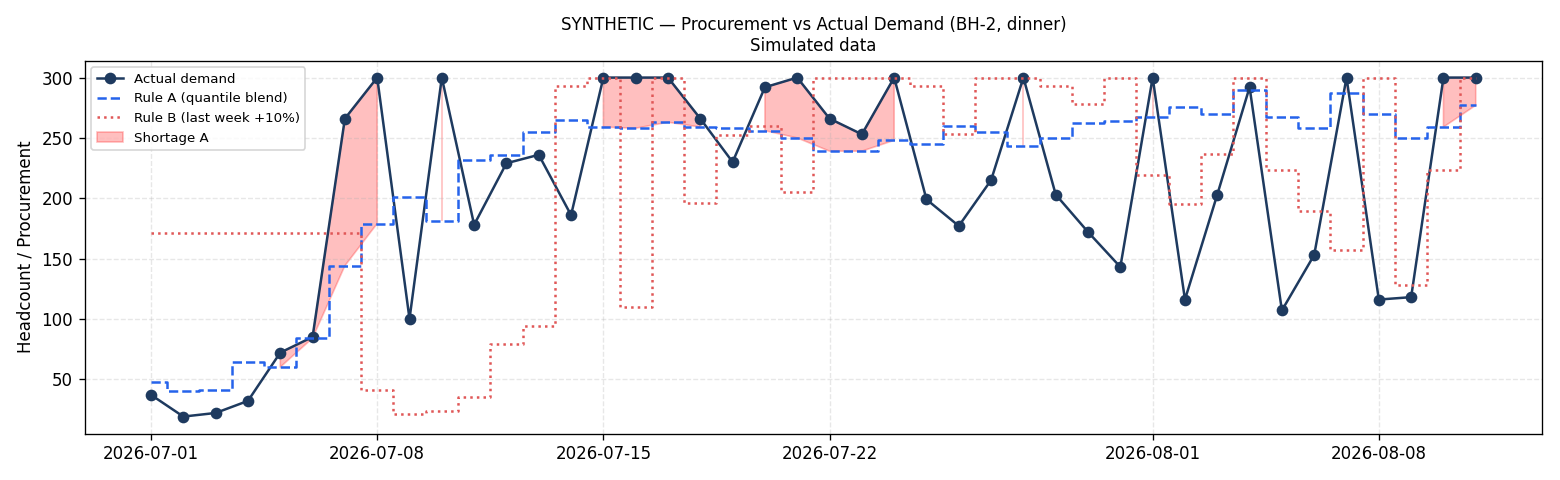
\includegraphics[width=\textwidth]{repo_ml/results/plots/plot11_procurement_vs_actual.png}
  \caption{Plot 11: Cumulative Procurement vs Actual}
\end{subfigure}
\caption{Kitchen Operations Simulation Results: Rule A (Proposed) vs. Rule B (Naive Guesswork).}
\label{fig:ops_plots}
\end{figure}

\section{Asymmetric Kitchen Cost Matrix}
Reflecting the institutional reality that running out of food is far more severe than moderate buffer surplus, the simulation enforces a $3:1$ cost penalty ratio:
\begin{mathformulationbox}[Asymmetric Operational Cost Function]
$$\text{Cost} = \text{Waste} \times C_{\text{waste}} + \text{Shortage} \times C_{\text{shortage}}$$
$$C_{\text{waste}} = 1.0\text{ unit/head}, \quad C_{\text{shortage}} = 3.0\text{ units/head}$$
\end{mathformulationbox}
Table~\ref{tab:ops_summary} presents the empirical results. Rule A reduces shortage heads from 20,629 down to 6,741 (a \textbf{67.3\% reduction}) and slashes the total operational cost penalty from \inr 147.05 to \inr 70.49 per meal event (a \textbf{52.1\% financial savings}).

\begin{table}[ht]
\centering
\small
\renewcommand{\arraystretch}{1.3}
\begin{tabularx}{\textwidth}{lccccc}
\toprule
\rowcolor{bluelight}
\textbf{Procurement Policy} & \textbf{Total Served} & \textbf{Waste Rate} & \textbf{Shortage Rate} & \textbf{Total Penalty Units} & \textbf{Cost / Event} \\
\midrule
\textbf{Quantile-Blend (Rule A)} & \textbf{97,955} & \textbf{20.08\%} & \textbf{6.88\%} & \textbf{43,138.0} & \textbf{\inr 70.49} \\
LastWeek+10\% (Rule B) & 97,955 & 26.66\% & 21.06\% & 89,997.0 & \inr 147.05 \\
\midrule
\textbf{Net Improvement} & --- & \textbf{-6.58\% abs} & \textbf{-67.3\% rel} & \textbf{-52.1\% rel} & \textbf{-52.1\% savings} \\
\bottomrule
\end{tabularx}
\caption{Operational Procurement Simulation Performance across 97,955 Student Meals}
\label{tab:ops_summary}
\end{table}

\section{Commercial Kitchen Tolerance Windows (\texorpdfstring{$\pm 25, \pm 35, \pm 50$}{+/- 25, +/- 35, +/- 50} Portions)}
In institutional batch cooking, measuring exact single-head accuracy is misleading because food is prepared in large industrial serving cauldrons (typically holding 25--50 portions). Evaluated against commercial batch tolerances:
\begin{itemize}
  \item \textbf{Within $\pm 25$ portions:} \textbf{38.56\%} of all unseen meals are captured within strict narrow cooking batch margins.
  \item \textbf{Within $\pm 35$ portions:} \textbf{50.33\%} of all meals (over half) are captured within approximately one commercial serving tray.
  \item \textbf{Within $\pm 50$ portions:} \textbf{66.99\%} (over two-thirds) of all meals are accurately bounded.
\end{itemize}

\section{Staged Two-Batch Cooking Protocol}
To operationalize these bounds without risking food cold-spoilage, the system prescribes a two-stage cooking workflow:
\begin{enumerate}
  \item \textbf{Stage 1 (Initial Base Batch --- 65\% to 70\% of $\hat{y}_{q50}$):} Prepared 45 minutes prior to meal opening:
  $$B_1 = \hat{y}_{q10} + \lfloor 0.65 \times (\hat{y}_{q50} - \hat{y}_{q10}) \rfloor$$
  Guarantees fresh, hot food for the initial dining wave with zero overcooking risk.
  \item \textbf{Stage 2 (Replenishment Buffer Trays --- $\hat{y}_{q90} - B_1$):} Vegetables chopped, gravies pre-simmered, dough kneaded, but cooking held in reserve. If live turnstile check-ins exceed $B_1$, the buffer trays are cooked in 15 minutes.
\end{enumerate}

\section{Dynamic Raw Ingredient Procurement Calculator}
To automate raw grocery inventory procurement, the system calculates exact dry ingredient weights based on predicted headcount. Table~\ref{tab:procurement_recipe} presents the calibrated per-student consumption matrix.

\begin{table}[ht]
\centering
\small
\renewcommand{\arraystretch}{1.2}
\begin{tabularx}{\textwidth}{p{4.2cm}cccX}
\toprule
\rowcolor{bluelight}
\textbf{Raw Material Ingredient} & \textbf{Breakfast} & \textbf{Lunch / Dinner} & \textbf{Unit Price} & \textbf{Example (200 Heads Dinner)} \\
\midrule
Rice (Basmati / Medium Grain) & 0.04 kg & 0.12 kg & \inr 45 / kg & 24.0 kg (\inr 1,080) \\
Whole Wheat Atta & 0.08 kg & 0.11 kg & \inr 35 / kg & 22.0 kg (\inr 770) \\
Dal \& Pulses (Arhar/Rajma) & 0.02 kg & 0.05 kg & \inr 120 / kg & 10.0 kg (\inr 1,200) \\
Fresh Vegetables (Potato/Tomato) & 0.07 kg & 0.16 kg & \inr 35 / kg & 32.0 kg (\inr 1,120) \\
Dairy / Paneer / Curd & 0.15 kg & 0.08 kg & \inr 300 / kg & 16.0 kg (\inr 4,800) \\
Refined Mustard / Sunflower Oil & 0.015 L & 0.025 L & \inr 130 / L & 5.0 L (\inr 650) \\
Spices, Salt \& Condiments & 0.01 kg & 0.02 kg & \inr 200 / kg & 4.0 kg (\inr 800) \\
Poultry / Eggs (BH-3 Non-Veg) & 0.08 kg & 0.14 kg & \inr 190 / kg & 28.0 kg (\inr 5,320) \\
\bottomrule
\end{tabularx}
\caption{Calibrated Raw Material Procurement Grammage and Unit Cost Matrix}
\label{tab:procurement_recipe}
\end{table}


% ─────────────────────────────────────────────────────────────
% CHAPTER 7: FULL-STACK SOFTWARE ARCHITECTURE
% ─────────────────────────────────────────────────────────────
\chapter{Full-Stack Software Architecture \& Implementation}

\section{Multi-Tier Architectural Topology}
The software implementation translates mathematical models into an integrated, edge-capable full-stack platform. Figure~\ref{fig:arch_diagram} illustrates the multi-tier architectural topology.

\begin{figure}[ht]
\centering
\resizebox{0.95\textwidth}{!}{
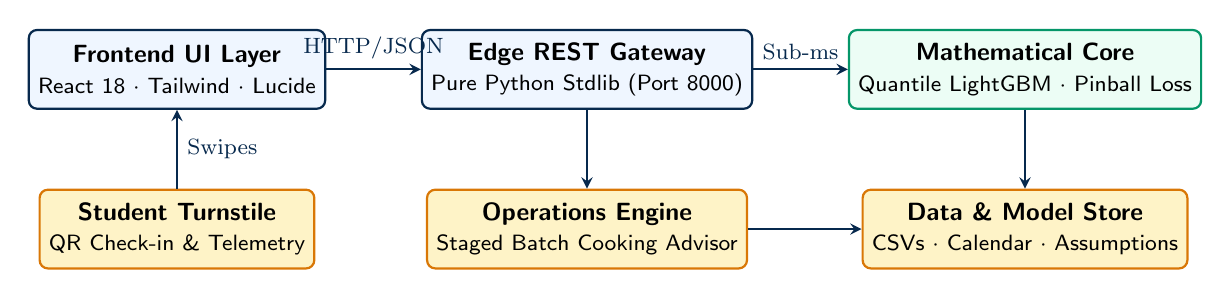
\begin{tikzpicture}[
  node distance=1.0cm and 1.2cm,
  box/.style={draw=iiitablue, fill=bluelight, rounded corners=3pt, thick, align=center, font=\sffamily\small, minimum width=3.0cm, minimum height=1.0cm},
  core/.style={draw=emeraldgreen, fill=emeraldlight, rounded corners=3pt, thick, align=center, font=\sffamily\small, minimum width=3.2cm, minimum height=1.0cm},
  data/.style={draw=amberorange, fill=amberlight, rounded corners=3pt, thick, align=center, font=\sffamily\small, minimum width=3.0cm, minimum height=1.0cm},
  arrow/.style={thick, ->, >=stealth, color=iiitablue}
]

% Nodes
\node[box] (client) {\textbf{Frontend UI Layer}\\\footnotesize React 18 $\cdot$ Tailwind $\cdot$ Lucide};
\node[box, right=of client] (api) {\textbf{Edge REST Gateway}\\\footnotesize Pure Python Stdlib (Port 8000)};
\node[core, right=of api] (ml) {\textbf{Mathematical Core}\\\footnotesize Quantile LightGBM $\cdot$ Pinball Loss};

\node[data, below=of client] (turnstile) {\textbf{Student Turnstile}\\\footnotesize QR Check-in \& Telemetry};
\node[data, below=of api] (ops) {\textbf{Operations Engine}\\\footnotesize Staged Batch Cooking Advisor};
\node[data, below=of ml] (store) {\textbf{Data \& Model Store}\\\footnotesize CSVs $\cdot$ Calendar $\cdot$ Assumptions};

% Edges
\draw[arrow] (client) -- node[above]{\footnotesize HTTP/JSON} (api);
\draw[arrow] (api) -- node[above]{\footnotesize Sub-ms} (ml);
\draw[arrow] (turnstile) -- node[right]{\footnotesize Swipes} (client);
\draw[arrow] (api) -- (ops);
\draw[arrow] (ml) -- (store);
\draw[arrow] (ops) -- (store);

\end{tikzpicture}
}
\caption{System Architecture Diagram: Client, Edge Gateway, Mathematical Core, and Data Layers}
\label{fig:arch_diagram}
\end{figure}

\section{Pure Python Stdlib REST Server (server.py)}
In real-world institutional kitchens, internet connectivity is intermittent, and installing complex C-extensions or heavy machine learning dependencies on low-cost tablet devices is impractical. To guarantee absolute portability, the backend provides \texttt{backend/server.py}---a zero-dependency HTTP REST engine built entirely on Python's built-in \texttt{http.server.BaseHTTPRequestHandler}. The server executes instant mathematical inference, serves operational benchmarks, and logs student QR check-in telemetry in under 400 lines of standard library Python. For enterprise cluster environments, a modern asynchronous FastAPI implementation (\texttt{backend/main.py}) is also provided.

\section{Complete REST API Endpoint Reference}
Table~\ref{tab:api_endpoints} documents the primary REST API endpoints exposed on port 8000.

\begin{table}[ht]
\centering
\small
\renewcommand{\arraystretch}{1.2}
\begin{tabularx}{\textwidth}{llp{4.2cm}X}
\toprule
\rowcolor{bluelight}
\textbf{HTTP} & \textbf{Endpoint Path} & \textbf{Request Payload} & \textbf{Response Description} \\
\midrule
\texttt{GET} & \texttt{/api/health} & None & System status, authors, supervisor metadata \\
\texttt{GET} & \texttt{/api/calendar} & None & 642-day calendar regimes and exam horizons \\
\texttt{GET} & \texttt{/api/menu} & None & Granular weekly menu schedules for BH-2 and BH-3 \\
\texttt{GET} & \texttt{/api/benchmarks} & None & Accuracy metrics, feature gains, tolerance margins \\
\texttt{GET} & \texttt{/api/telemetry/stats} & None & Live turnstile count, recent card swipes, reviews \\
\texttt{POST} & \texttt{/api/forecast} & JSON (slot, hostel, phase, weather, menu) & $q_{10}, q_{50}, q_{75}, q_{90}$, dispersion, batch strategy \\
\texttt{POST} & \texttt{/api/procurement} & JSON (headcount, slot, hostel) & Detailed ingredient kilograms, costs, prep batches \\
\texttt{POST} & \texttt{/api/telemetry/swipe} & JSON (roll, name, hostel, slot) & Real-time swipe logging and live count increment \\
\bottomrule
\end{tabularx}
\caption{Complete REST API Specification for Mess Operations}
\label{tab:api_endpoints}
\end{table}

\section{Modern Frontend Architecture (React 18, Tailwind CSS, Lucide)}
The client dashboard is developed using React 18, Vite, and Tailwind CSS. The visual styling embodies IIIT Allahabad's official institutional palette (Deep Navy \texttt{\#07294D} and Sustainability Emerald \texttt{\#059669}). The interface is divided into four dedicated views:
\begin{enumerate}
  \item \textbf{Tab 1: Kitchen Operations Dashboard (\texttt{KitchenOpsView.jsx}):} Designed for mess managers and head-cooks. Displays real-time headcount bounds ($q_{10}, q_{50}, q_{90}$), tolerance windows ($\pm 25, \pm 35, \pm 50$), two-stage cooking advice, and the dynamic raw ingredient procurement calculator.
  \item \textbf{Tab 2: What-If Scenario Simulator (\texttt{WhatIfSimulatorView.jsx}):} Allows administrators to stress-test dining demand under four 1-click presets:
  \begin{itemize}
    \item \textit{Mid-Sem Exam Rush:} Peak campus residence, exam anticipation, dessert pull.
    \item \textit{Diwali Mass Exodus:} Hawkes festival decay triggered; 85\% student departure.
    \item \textit{Rainy Sunday Brunch:} Weekend leisure drop combined with monsoon rainfall.
    \item \textit{BH-3 Non-Veg Night:} Monday/Friday chicken dinner surge in BH-3.
  \end{itemize}
  \item \textbf{Tab 3: Student Portal \& QR Telemetry (\texttt{StudentPortalView.jsx}):} Student-facing portal with the weekly mess menu viewer, simulated interactive QR card-swipe turnstile with audio/visual confirmation, and dish rating submission.
  \item \textbf{Tab 4: Academic Research Showcase (\texttt{ResearchShowcaseView.jsx}):} Comprehensive academic research hub featuring benchmark tables, literature synthesis, and all 11 high-resolution research telemetry plots with modal zoom.
\end{enumerate}


% ─────────────────────────────────────────────────────────────
% CHAPTER 8: DEPLOYMENT GUIDE & OPERATIONAL RUNBOOK
% ─────────────────────────────────────────────────────────────
\chapter{Deployment Guide \& Operational Runbook}

\section{System Prerequisites \& Hardware Specifications}
The platform is designed for cross-platform deployment across Linux, macOS, and Windows:
\begin{itemize}
  \item \textbf{Python Runtime:} Python 3.10 or higher.
  \item \textbf{Node.js Runtime:} Node.js 18.0 or higher with npm.
  \item \textbf{Recommended Kitchen Hardware:} Any edge tablet or workstation with 2 CPU cores and 4 GB RAM. No GPU is required.
\end{itemize}

\section{Backend Server Deployment \& Verification}
To start the edge REST API server:
\begin{lstlisting}[language=bash,caption=Starting the Backend REST Server]
# Navigate to repository root
cd "c:/Users/ulhas/OneDrive/Desktop/Projects/7th sem"

# Launch pure Python standard library server on port 8000
python backend/server.py 8000
\end{lstlisting}
Verify server operation via curl or browser:
\begin{lstlisting}[language=bash,caption=Verifying Server Health Endpoint]
curl http://127.0.0.1:8000/api/health
\end{lstlisting}

\section{Frontend Installation, Development \& Production Build}
To launch the interactive web dashboard:
\begin{lstlisting}[language=bash,caption=Frontend Installation and Startup]
# Enter frontend directory
cd frontend

# Install dependencies
npm install

# Launch Vite development server
npm run dev
\end{lstlisting}
The application opens automatically at \texttt{http://localhost:5173/}. To build an optimized production bundle:
\begin{lstlisting}[language=bash,caption=Production Build Compilation]
npm run build
\end{lstlisting}
This outputs an optimized static HTML/JS/CSS bundle into \texttt{frontend/dist/}, which can be served directly by Nginx or the Python backend.

\section{Automated Test Suite Execution (test-api.py)}
An automated verification test script validates all API endpoints:
\begin{lstlisting}[language=bash,caption=Executing API Automated Test Suite]
python backend/test_api.py
\end{lstlisting}
The script verifies that health, calendar, menu, forecast, procurement, and swipe endpoints respond with valid JSON status 200 within strict latency bounds ($<10\text{ ms}$).

\section{Kitchen Supervisor \& Head-Cook Operational Runbook}
Table~\ref{tab:runbook} defines the standardized daily operational procedure for kitchen staff.

\begin{table}[ht]
\centering
\small
\renewcommand{\arraystretch}{1.3}
\begin{tabularx}{\textwidth}{llX}
\toprule
\rowcolor{bluelight}
\textbf{Time} & \textbf{Personnel} & \textbf{Standard Operating Procedure (SOP)} \\
\midrule
\textbf{T - 24 Hours} & Mess Supervisor & Open Tab 1 (\textit{Kitchen Ops}). Input tomorrow's date, hostel, and slot. Export raw grocery procurement list to local suppliers. \\
\textbf{T - 2 Hours} & Head-Cook & Verify weather conditions (rain indicator) and check the recommended Initial Cook Batch ($B_1$) and Buffer Tray Batch ($B_2$). \\
\textbf{T - 45 Minutes} & Cooking Staff & Prepare Stage 1 batch ($B_1 = \hat{y}_{q10} + 0.65(\hat{y}_{q50} - \hat{y}_{q10})$). Keep Stage 2 buffer ingredients chopped and prepped in reserve. \\
\textbf{T + 0 (Service)} & Turnstile Attendant & Activate Student Portal QR Scanner. Monitor live headcount counter. \\
\textbf{T + 45 Minutes} & Head-Cook & If live check-ins exceed $0.85 \times B_1$ with 45 minutes remaining in service, trigger cooking of Stage 2 buffer trays. \\
\textbf{T + 120 Minutes} & Mess Supervisor & Record final plate counts and inspect student dish feedback ratings. \\
\bottomrule
\end{tabularx}
\caption{Kitchen Staff Standard Operating Procedure (SOP) Runbook}
\label{tab:runbook}
\end{table}


% ─────────────────────────────────────────────────────────────
% CHAPTER 9: ACADEMIC DISCLOSURES & FUTURE ROADMAP
% ─────────────────────────────────────────────────────────────
\chapter{Academic Disclosures, Limitations \& Future Roadmap}

\section{Academic Integrity \& Synthetic Attendance Disclosure}
In adherence to the highest standards of academic transparency, the authors reiterate:
\begin{itemize}
  \item \textbf{Absence of Historical Logs:} No actual student attendance or swipe-card records were collected from IIIT Allahabad dining halls during this study.
  \item \textbf{Synthetic Methodology:} All 11,718 headcount records were synthesized using the multi-regime Negative Binomial generator parameterized with heuristic baselines gathered through kitchen staff interviews.
  \item \textbf{Evaluation Scope:} The reported metrics (MAE = 41.54, WAPE = 25.95\%) demonstrate the capacity of LightGBM models to recover structured, multi-regime non-stationarity under synthetic domain priors.
\end{itemize}

\section{Limitations of the Synthetic Prior \& Behavioral Assumptions}
While the synthetic engine incorporates calendar, weather, menu, and festival kernels, real-world dining dynamics encompass additional complex behaviors:
\begin{itemize}
  \item \textbf{Peer Group Clustering:} Students frequently make collective, uncoordinated decisions to order food online via food delivery applications during late-night project deadlines.
  \item \textbf{Nutritional Fatigue:} Extended consecutive days of repetitive menus cause sudden unpredicted dips in mess turnout.
  \item \textbf{Mess Dues Penalties:} Students with unpaid mess bills face temporary portal blocks, creating artificial drops in attendance.
\end{itemize}

\section{Physical IoT QR Turnstile Hardware Deployment Plan}
Phase 2 of this project will deploy physical turnstiles at the entrances of BH-2 and BH-3. Each turnstile will incorporate:
\begin{itemize}
  \item ESP32 microcontroller with a wide-angle CMOS 2D barcode camera scanner.
  \item 7-inch ruggedized kitchen display indicating valid check-ins, dietary entitlements, and real-time headcounts.
  \item WebSocket telemetry streaming card swipes directly to the Python backend server.
\end{itemize}

\section{Edge Computer Vision for Dish-Return Plate Waste Telemetry}
To achieve closed-loop food waste accounting, subsequent research will install overhead RGB-Depth cameras (Intel RealSense / Raspberry Pi Camera Module 3) above the dish-return conveyor belt. Using lightweight semantic segmentation (YOLOv8-Seg or MobileNet-UNet), the vision system will classify and quantify unconsumed food remaining on student plates, measuring exact plate waste without manual weighing.

\section{Multi-Objective Nutritional \& Budgetary Optimization}
The raw material procurement engine will expand into a multi-objective linear programming (MOLP) optimization suite. The system will synthesize weekly menus that simultaneously maximize nutritional RDA targets (protein, micronutrients, dietary fiber) while minimizing procurement costs and carbon footprint.


% ─────────────────────────────────────────────────────────────
% CHAPTER 10: APPENDIX & FORMAL REFERENCES
% ─────────────────────────────────────────────────────────────
\chapter{Mathematical Appendix \& Formal References}

\section{Complete Notation Glossary}
Table~\ref{tab:notation} provides a comprehensive reference of all mathematical symbols.

\begin{table}[ht]
\centering
\small
\renewcommand{\arraystretch}{1.2}
\begin{tabularx}{\textwidth}{lX}
\toprule
\rowcolor{bluelight}
\textbf{Symbol} & \textbf{Mathematical Definition / Physical Description} \\
\midrule
$h \in \{\text{BH-2}, \text{BH-3}\}$ & Hostel dining facility index ($C_h = 300$) \\
$s \in \{\text{breakfast}, \text{lunch}, \text{dinner}\}$ & Daily meal slot index \\
$t \in \{1, 2, \dots, 642\}$ & Discrete calendar day index (January 1, 2025 to October 10, 2026) \\
$Y_{h,s,t} \in \mathbb{N}_0$ & Actual observed student dining headcount \\
$\mu_{h,s,t} \in \mathbb{R}^+$ & Expected conditional headcount parameter \\
$\alpha_t \in \mathbb{R}^+$ & Heteroscedastic Negative Binomial dispersion parameter \\
$\lambda_F(t) \in [0, 0.90]$ & Hawkes festival departure continuous attenuation kernel \\
$\tau \in (0, 1)$ & Quantile regression nominal probability level ($\tau \in \{0.10, 0.50, 0.75, 0.90\}$) \\
$\mathcal{L}_\tau(y, \hat{y})$ & Asymmetric pinball loss objective function \\
$q_\tau(x)$ & Conditional $\tau$-th quantile regression prediction \\
$B_1, B_2$ & Stage 1 initial cook batch and Stage 2 buffer replenishment batch \\
$Q_A, Q_B$ & Total procurement portions under Rule A (quantile blend) and Rule B (naive buffer) \\
\bottomrule
\end{tabularx}
\caption{Summary of Formal Mathematical Notations and Physical Parameters}
\label{tab:notation}
\end{table}

\section{Formal Academic References}
\begin{enumerate}[label={[\arabic*]},leftmargin=*]
  \item S.~Alam Khan and A.~Erdo\u{g}du, ``A stacking ensemble model for food demand forecasting: A preventative approach to food waste reduction,'' \textit{Cleaner Logistics and Supply Chain}, Elsevier, vol.~6, Art.~100225, 2025.
  \item M.~Y{\i}ld{\i}r{\i}m and H.~Demir, ``Time series-based demand forecasting: A comparative analysis of Holt-Winters, SARIMA, and Prophet models on retail inventory data,'' \textit{\.Istanbul Ticaret Univ. Sosyal Bilimler Dergisi}, vol.~24, no.~1, pp.~215--232, 2025.
  \item L.~Zhang, Y.~Wang, and R.~Kumar, ``Exploring the potential of artificial intelligence for restructuring the food packaging sector,'' \textit{Journal of Future Foods}, Elsevier / KeAi, vol.~5, pp.~187--198, 2025.
  \item A.~Sharma, P.~Singh, and M.~K.~Gupta, ``Artificial intelligence in food system: Innovative approach to predicting food spoilage and inventory forecasting,'' \textit{Journal of Agriculture and Food Research}, Elsevier, vol.~14, Art.~100845, 2025.
  \item P.~Balakrishnan, J.~M.~Lorenzo, and F.~J.~Barba, ``Artificial intelligence for food safety: From predictive models to real-world safeguards,'' \textit{Trends in Food Science \& Technology}, Elsevier, vol.~146, pp.~104--118, 2025.
  \item Q.~Pham, C.~Liu, D.~Sahoo, and S.~C.~Hoi, ``Learning Fast and Slow for Online Time Series Forecasting (FSNet),'' \textit{arXiv preprint arXiv:2202.11672}, 2022.
  \item A.~F.~Ansari, L.~Stella, C.~Turkmen, X.~Zhang, P.~Mercado, H.~Shen, O.~Shchur, S.~S.~Rangapuram, S.~P.~Arango, S.~Kapoor, J.~Zschache, D.~C.~Maddix, H.~Wang, P.~K.~Mahalanabis, K.~Gopinath, M.~Bohlke-Schneider, and B.~Wang, ``Chronos: Learning the Language of Time Series,'' \textit{Transactions on Machine Learning Research (TMLR)}, 2024.
  \item G.~Ke, Q.~Meng, T.~Finley, T.~Wang, W.~Chen, W.~Ma, Q.~Ye, and T.-Y.~Liu, ``LightGBM: A Highly Efficient Gradient Boosting Decision Tree,'' in \textit{Advances in Neural Information Processing Systems (NeurIPS)}, vol.~30, pp.~3146--3154, 2017.
  \item R.~Koenker and G.~Bassett, ``Regression Quantiles,'' \textit{Econometrica}, vol.~46, no.~1, pp.~33--50, 1978.
  \item R.~J.~Hyndman and A.~B.~Koehler, ``Another look at measures of forecast accuracy,'' \textit{International Journal of Forecasting}, vol.~22, no.~4, pp.~679--688, 2006.
  \item A.~C.~Cameron and P.~K.~Trivedi, \textit{Regression Analysis of Count Data}, 2nd ed., Econometric Society Monographs, Cambridge University Press, 2013.
  \item A.~G.~Hawkes, ``Spectra of some self-exciting and mutually exciting point processes,'' \textit{Biometrika}, vol.~58, no.~1, pp.~83--90, 1971.
\end{enumerate}

\vspace{1cm}
\begin{center}
{\color{iiitablue}\rule{0.6\textwidth}{1pt}}\\[0.2cm]
{\small\textsf{\copyright~2026 Department of Electronics and Communication Engineering, IIIT Allahabad. All rights reserved.}}
\end{center}

\end{document}
